\documentclass[11pt,UKenglish,a4paper,twoside]{report}
\usepackage{graphicx}
\usepackage{mystyle}
%\graphicspath{ {img/} } %bruker heile paths sidan pandoc ikkje støtter \graphicspath{}

\title{	
	{\large Flashing Large Mammals}\\
	{\small Quantifying the effect of white LED flash on camera trapping detection rates}\\
	{~}\\
	{\large Centre for Ecological and Evolutionary Synthesis}\\
	{
\includegraphics[scale=0.5]{./img/MN_IMBV_A_ENG.png}}\\
%	{\includegraphics[scale=0.5]{./img/CEES.png}}\\	
}
\author{Torgeir Holmgard Valle}
\date{\today}

%Det finnes diverse gode interaktive tegneprogrammer, for eksempel
%AdobeIllustrator, Inkscape, GIMP og paint.net, samt et meget godt deklarativt tegne-program:MetaPost.

\includeonly{tex/intro, tex/method, tex/results} 
\begin{document}

\maketitle

%\section*{Abstract}

Camera trapping is an increasingly important tool in animal ecology that is generally targeted towards large mammals, and especially large carnivores.
Nonetheless, the cameras are triggered by all large and medium-sized animal species in the area, and thus gathers valuable data on the whole ecological community, like their diel and seasonal activity patterns.
% And
White light flashes are sometimes utilized to get more detailed photos allowing for capture-recapture based population estimates for naturally marked species, like the Eurasian lynx (\textit{Lynx lynx}).
% But
However, the white light could function as a stressor or attractant for different species, which would affect density estimates. 
There is evidence of behavioural change in several mammal species, when exposed to a white flash, but quantifications on the detection rate of species are still lacking.

% In this study
Therefore, I investigated whether introducing an additional white LED camera trap (CT) at established CT sites affected the detection rates of the most common wild mammal species in the area. As CT flashes only are used while ambient lighting is low, I quantified the species' diel patterns in the process.

% I predicted 
I predicted that the detection rate of species with nocturnal and crepuscular activity patterns would be altered as a response to the white light stimuli, and that the extent of the effect would depend on the species' visual acuity. 

% What happened was
The results showed no significant effects of white LED flashes, when compared to IR flashes,
suggesting that white-flash cameras are suitable for studies using indices and capture-mark-recapture estimators. 

\thispagestyle{plain}

%\textit{Keywords:} 
%%Animal behaviour; % Tja, eit klart resultat av åtferd, men eg bruker liten tid på det i oppgåva
%camera trap;
%camera trap shyness; % To the point!
%monitoring bias; % To the point
%night-time photography; % Det er vertfall då det burde ha noko å sei
%diel activity; % Nå som eg har brukt så mykje tid på det
%density estimation; % Hovudgrunnen til å undersøke detection rates


%When in the abstract of an article, authors conclude an effect is “statistically equivalent,” the abstract should also include the equivalence bounds that are used to draw this conclusion.
%TODO Frå TOST-artikkelen til Daniel Lakens (2017)
%\chapter{Dedication}

To mum and dad
%\chapter{Acknowledgements}

I always assumed that writing a long text would be straightforward. One sits down and writes from start to finish, and then what remains to do is simply to check for misspellings.
However, writing this thesis, I've learned that this is far from the truth, as both my supervisors and myself had trouble understanding some of the sections I've written along the way.
Finally, after many attempts, my thesis is hopefully coherent for anyone wanting (or having) to read it.

Thanks to my supervisors Atle Mysterud, John Odden, Neri Thorsen and Inger Maren Rivrud.

Atle, thank you for making me focus on the positives and motivate me to keep going...
John, thank you for giving me the opportunity to work on a project related to lynx (although it evaded me... )
Neri, thank you for all the help with data wrangling and setting up my analyses. After a while I was able to understand your <codes>.
Inger Maren, thank you for the advice in writing...


Alle i CT-avdelinga til NINA: for behandling av data til oppgåva mi

Special mentioning: Solveig og Nina for problemløysing i 'nødstilfeller', rettleiing og å alltid ha vert tilgjengelig på telefon, tilogmed på fritid og ute i skog og mark med familie

During several hundred hours of field work, I was lucky enough to bring some friends along the way.
I want to thank all my friends that joined me for a day in the field, and a speciel thanks to Olav Rørstad, who joined me for several weeks. Two idiots were better than one, when the car got stuck in an uphill, snowy, dirt road (or two).

\tableofcontents
\listoffigures
\listoftables

% -- intro --
\chapter{Introduction}
%Bakgrunn
Estimating the number of animals is central in population ecology, and census methods have always been under development in order to get accurate, reliable ways of conducting surveys \autocite{morellet2011}.
%Estimeringstrøbbel
Direct observations are prone to undercounting, as many species are elusive and observer concentration dwindles over time. Telemetry studies can provide very detailed knowledge, but studies are usually limited in extent, as they are costly and invasive in nature \autocite{Ikeda2016}. %TODO Seier han dette om telemetry?
Distribution of medium sized and large mammals are therefore often based on proxy data such as harvest statistics, but such methods tend to be quite unreliable due to variable hunter effort. In particular for large carnivores, harvest may also be low or absent for periods where management targets are not obtained \autocite{morellet2011}.
 %AM: hele avsnittet må få på referanser


In recent years, automated camera traps (CT) have been developing fast, and become quite affordable \autocite{Burton2015}. 
CTs offer a consistent, standardised sampling method, and provide information about the presence, demography and behaviour of multiple species with a high temporal resolution \autocite{Ikeda2016}. 
CTs are traditionally used to study a single species in a specific study site, but they are increasingly seen as a tool for investigating multiple sympatric species, their interactions and diel patterns \autocite{Ikeda2016}. 
The underlying assumption is that CTs are unselective in which species they capture, or that biases in capture rates can be corrected for by using covariates in a statistical framework \autocite{Hofmeester2019}.  


Camera traps have been considered non-invasive, but can affect animal behaviour in several ways \cite{Meek2014a}, for example through detecting sounds from triggering camera, scents from human operators, the unfamiliar shape of the camera itself or the flash used in night-time \autocite{Wegge2004,Burton2015, Beddari2019}.
% IR and why white flash
During night time, CTs normally use infra-red (IR) light from an array of light-emitting diodes (LED) to photo capture animals, which is invisible to human eyes, but has been shown to be visible to several other mammals \autocite{Meek2014a, Meek2016}. 
However, the lack of sharpness and detail from IR photos limit the information we can retrieve from them, as for example individual variation in coat patterns (e.g. tigers (\textit{Panthera tigris}), jaguars (\textit{Panthera onca}) and lynx) which can be used in capture-mark-recapture models to accurately estimate population numbers \autocite{Meek2014a,Rovero2013}. 

Needing more photographic detail, white LED, as well as the original white xenon flashes, has been increasingly incorporated in CT surveys \autocite{Rovero2013}.
Xenon provides the sharpest photos due to a more powerful light \cite{Rovero2013}, but has the disadvantage of requiring long cool downs after each photo \autocite{Henrich2020}.

Naturally, white light is highly visible to all land dwelling mammals, and can therefore increase the number of CT aware animals \autocite{Glen2013a,Dryja2005}. The white light could even increase the chance of causing flash blindness in the passing animal \cite{Dryja2005}.
That could be detrimental, as studies using indices and capture-mark-recapture estimators must avoid altering animal behaviour during or between monitoring sessions, not to affect their detectability \autocite{Meek2014a}.
Therefore, there is a need to determine which species are influenced, and to what extent their detection rates are altered in comparison to IR flash CTs.
%flash and diel pattern
A CT's flash is used whenever natural light gets scarce. 
The darker it is, the stronger the white flash stimulus will be (because of dark habituated eyes).
Thus, white and IR flash CTs should in theory only differ in effect during night, and animal responses will depend on the species activity patterns (see below). 


% Eye morphology %%%%%%%%%%%%%%%%%

White light affects all photoreceptors in an animals retina \autocite{Dryja2005}, whereas IR flash only would affect those that are sensitive to IR wavelengths. 
A white flash can therefore increase the total number of CT aware animals.
The white light could be associated to human presence in the form of artificial light at night, and could trigger a response depending on the animal's relationship to humans.
Scavengers could be attracted to the light in search for garbage (food).
High conflict species, like the grey wolf (\textit{Canis lupus}), could be scared off, as high hunting pressure could select for shy and elusive individuals.
However, a quantification of the effects white flash CTs have on species detectability is still lacking, to the best of my knowledge.



%%%%% Morphological studies %%%%%%%%%%%%%%%%%%%%%%%%%%%
Eye morphology in animals differ with diel activity patterns, e.g. between nocturnal and diurnal species \autocite{Schmitz2010}. 
Most mammals vary less in eye morphology than other amniotes (birds and reptiles) \autocite{Schmitz2010, Hall2012}, but they have other adaptations to increase light sensitivity \autocite{Ollivier2004,Solovei2009}. 
Eye characteristics governing nocturnal behaviour could also affect a species' response to the white flash. More light sensitive eyes will react stronger to the white flash, especially considering that rod cells (low-light sensitivity) take longer to depolarize than cone cells (visual acuity and color distinction) \autocite{Dryja2005}.
Thus, nocturnal and crepuscular (active at twilight) mammals could experience glare or flash blindness.
Flash blindness can cause spatial disorientation or loss of situation awareness in humans \autocite{Nakagawara2001}, but as most mammals rely less on optical senses than humans, they might not react as strongly.
I argue that relative visual acuity is correlated with a species' reliance on sight, and it has been used in previous studies as a way to compare animals of disparate size \autocite{Hall2012}. 

%% Flytta til diskusjon %%%%%%%%%%%%%%%%%%%%%%%%%%%%%%%%%%
%"The ratio of corneal diameter to axial length of the eye is a useful measure of relative sensitivity and relative visual acuity that has been used in previous studies as a way to compare animals of disparate size."
%Relative acuity is given in table 1.1 as axial length divided by corneal diameter.
%The higher the value of relative acuity, the higher the hypothetical importance of sight for each species.


%%%%%%%%%%%%%%%%%%%%%%%%%%%%%%%%%%%%%%%%%%%%%%%%%%%%%%%%%%%
In this study, I will quantify how the usage of white LED flash affects the detection rate of the most common large mammal species in an area in southeastern Norway.
White LED CTs have similar recovery speeds to that of regular IR CTs, as both utilize LED flashes, which makes them well fit for meaningful comparison.
A subgoal is to quantify the species' activity patterns, providing data on nine sympatric mammalian species at high northern latitudes, and how their diel patterns change along the seasons.
Mammalian diel patterns can be categorized into diurnal, nocturnal, crepuscular (active at twilight), and cathemeral (active throughout the day) \autocite{Ikeda2016}.
In their CT study of seasonal and diel activity patterns, \textcite{Ikeda2016} strictly defined a species as cathemeral when no differences were observed in the photographic frequencies among day, night and twilight. Since this also is a CT study, I will use the same definition.

I have restricted the analysis to all wild species observed at least 50 independent times during my survey, which totaled nine species.
There were three cervids (roe deer (\textit{Capreolus capreolus}), moose (\textit{Alces alces}) and red deer (\textit{Cervus elaphus})),
four carnivores, of which two were mustelids (badger (\textit{Meles meles}), European pine marten (\textit{Martes martes})), one was canid (red fox (\textit{Vulpes vulpes})), one was felid (lynx), 
and two were members of the clade Glires; one rodent (red squirrel (\textit{Sqiurus vulgaris})), and one lagomorph (mountain hare (\textit{Lepus timidus})).
The species will be grouped by taxonomic relationships in results and discussion, assuming closely related species to have similar sensory anatomy (e.g. visual acuity), and therefore similar experiences of being exposed to a white flash during night time. %I will use data from the supplementary material of Hall et al. (2012) to discuss the relevance visual acuity can have on mammals reaction to white flashes.
Squirrels and hares are more distantly related than the two other groupings I've presented, and as such should be expected to have larger differences in their sensory anatomy. 
%%%%%%%%%%%%%%%%%%%%%%%%%%%%%%%%%%%%%%%%%%%%%%%%%%%%%%%%%%%
I predict usage of white LED flash will stress nocturnal and crepuscular species, and therefore lower their detection rates. The effect will likely be stronger for species with high relative visual acuity (lynx, pine martens) than low relative visual acuity (badgers).



%%%%% Cut from the morphology part %%%%%%%%%%%%%

%The eyes of crepuscular and cathemeral mammals are more similar to those of nocturnal than diurnal mammals, possibly due to the highly developed senses of hearing, smell and their tactile vibrissae, minimizing the evolutionary pressure of eyes that work well during daylight \autocite{Hall2012}. %TODO and Solovei2009? At least she talked about the plasticity of re-evolving rod cell structure to the normal diurnal structure.








% -- method --
\chapter{Method and materials}


\section{Study species} %Usikker på om eg skal ha med
%\subsubsection{Rev}  ?

%We also collated information on average body and home range sizes for a subset of species surveyed in the reviewed studies in order to better quantify the functional diversity of wildlife being sampled by CTs and to evaluate the degree to which CT methodologies were tailored to focal species. Burton 2015

The species I'll focus on in this thesis are the species that most frequently was observed \emph{(>50 events)}, excluding farmed animals (e.g. cattle), humans and dogs, and grouped categories of animals (e.g. birds).
Given that the decisions on camera placement (height and angle) were made with the aim on photo capturing lynx(), I have also excluded smaller species from the analysis.
% Idea sprung from reading Meek 2014 guiding principles; Height of camera and, distance to centre of detection zone or lure. Growing skeptical to the validity of my argument now that I know about the random effect in models. As I argued in my own notes when reading the Meek article I don't think I need to "take these biases into consideration" because I'm trying to detect differences between the same cameras.
This includes three species, squirrel(), hare() and European pine marten\textit{(Martes martes)}. 
Though they showed up frequently on many locations, there are inevitably some cameras that are too biased towards larger animals, resulting in an inconsistency of their detection rates. 
In turn, it is difficult to distinguish whether the species was affected by the white LED or not, as they could have triggered the camera, but already escaped the frame. %TODO må tygge litt på det argumentet.

In the end, the species I have used in my analyses are roe deer\textit{()}, red fox\textit{()}, badger\textit{(Meles meles)}, moose\textit{()}, red deer\textit{(Cervus elaphus)} and lynx. 

\section{Study area} %TODO 
%mogleg å kjøre ein fin overgang fra intro til study area? Study area valt pga dårlige snøforhold -> vanskelig å gjere spor-tellinger (\cite{Odden2015})


%https://klimaservicesenter.no/faces/desktop/article.xhtml?uri=klimaservicesenteret/klimaprofiler/klimaprofil-oslo-og-akershus
%https://klimaservicesenter.no/faces/desktop/article.xhtml?uri=klimaservicesenteret%2Fklimaprofiler%2Fklimaprofil-buskerud  
The study area (59.36-60.47° N, 9.43-10.91° E) %berre eit grovt overslag
extends over much of the southeastern parts of Norway in counties Flå, Krødsherad, Sigdal, Ringerike, Modum, Hole, Lier, Øvre Eiker, Asker, Oslo, Enebakk, Indre Østfold, Våler, Råde, Moss, Frogn and Vestby.
The climate has a continental character due to rain shadows of the mountain ridges from the west. 

The mean annual temperatures ranges from 2-6\celsius  and precipitation lies between 700-1500mm (\cite{Moen1999}). 
Topography is predominantly flat towards the south, and more rugged and elevated towards the north. The landscape is a mosaic of forest and agricultural areas, divided with a wide network of gravel roads.
The area is situated in the southern boreal and the boreonemoral zones. %Må finne oppdaterte data (frå Norges vassdrags- og energidirektorat, 2019?)

Norway spruce (\textit{Picea abies}) and Scots pine (\textit{Pinus sylvestris}) make up the dominating boreal coniferous forests, with frequent presence of silver birch (\textit{Betula pendula}) and downy birch (\textit{Betula pubescens}), then aspen (\textit{Populous tremula}), alder (\textit{Alnus incana}) and black alder (\textit{Alnus glutinosa}).

Growing season length 170 - 190 days (Moen, 1999, map 6, s.21) %må finne oppdaterte data
Snow cover length												%må finne oppdaterte data %TODO

Most cameras were set in forest areas, usually by a tractor path or human trail, sometimes by animal paths. Their distance from houses or roads varied to a large extent, and some areas were logged (ved Vansjø) and even greatly changed under development of new infrastructure (toglinje på nordligste kamera ~1255)


\section{Study design} %TODO
For the study I chose 60 already established camera sites with infrared light(Reconyx and Browning models), in order to have a reference of capture frequencies. The cameras had been installed on trees 1-3 meters from human or tractor paths, 40-120 cm above ground level, with the original aim to photo capture lynx (\cite{Odden2015}). 
I divided the sites randomly into three groups of 20 cameras. Cameras in group A remained unchanged, whilst group B and C were equipped with an additional white LED camera (Reconyx PC850) in alternating 3 month-periods, as shown in figure\vref{fig:exp_set}.

\begin{figure}
    \begin{center}
    	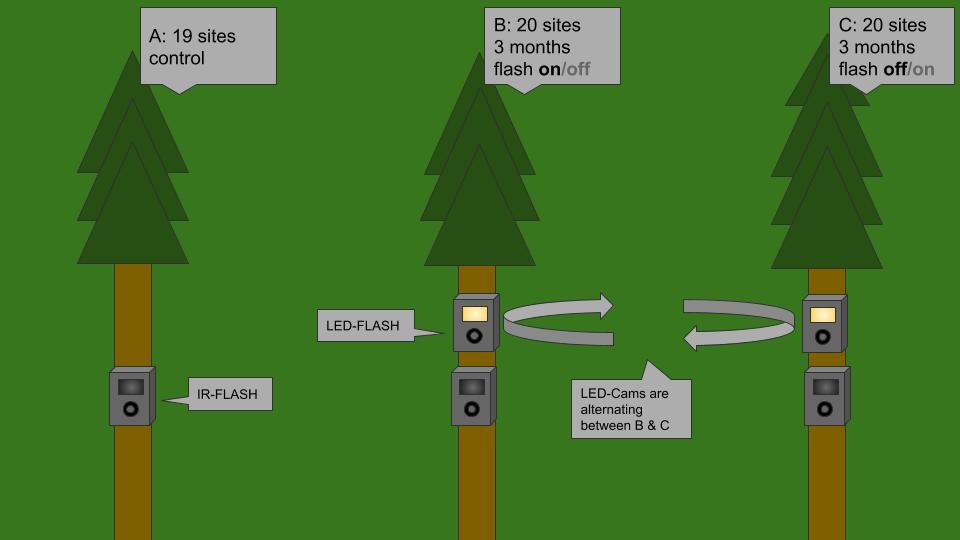
\includegraphics[scale=0.3]{experiment_setup} %insert figure of groups     
    \end{center}
    	\caption{Experiment setup}
    \label{fig:exp_set}
\end{figure}


The preinstalled cameras were set up and handled by people from the Norwegian Institute of Nature Research (NINA) and --- at the sites further from Oslo  --- by members of the Norwegian Hunters and Fishers Society (NJFF). 
%as a conflict mitigating strategy. %%Kan kuttes. Evt må det forklares
The installation of the cameras did not follow a strict protocol, nor were their locations chosen randomly. The overall placement was systematic as decided by NINA, then there was a deliberately-biased placement of the CTs put up in areas where the individual handler deemed it most likely to photograph lynx, and hence, based on a combination of site accessibility and expectations of animal occurence %(\cite{Burton2015} ). %TODO vask språket

%\emph{presence of natural or artificial attractants may draw animals in to a CT} \cite{Burton2015}.

As shown in figure\vref{fig:exp_set}, I set up all white LED cameras above the cameras already in place. 
However, at the particular site shown in figure\vref{fig:cam_ex_c} the infrared camera had been installed so far above ground level that I chose to position the white LED camera below the camera already in place. %endra på av Atle, men kan vaskas ytterligere 
For the periods without white flash treatment, I moved the cameras to their next site. However, the boxes installed on the trees remained (see figure \ref{fig:cam_ex_d}).
First, I equipped Group B with white LED in a 3 week period from January - February 2019. The boxes remained untill the end of the experiment. Group C, on the other hand, had no extra boxes before the start of the second period in May 2019 (i.e. remained identical to the control group A untill May).


I visited sites of group B and C at least once every three months in order to move the LED cameras. For convenience I visited sites of group A less often. %Her trengs ein språkleg endring
However, as the cameras were part of other, ongoing projects, they were occasionally visited by other workers from NINA to retreive the Secure Digital memory cards (hereby SD Cards) for data. %write in full on first mention (-Atle)
This was mostly the case for sites close to, and south of, Oslo, or rather, the cameras not normally operated by members of the NJFF.



\begin{figure}
		\begin{subfigure}{.5\textwidth}
		  \centering
		  	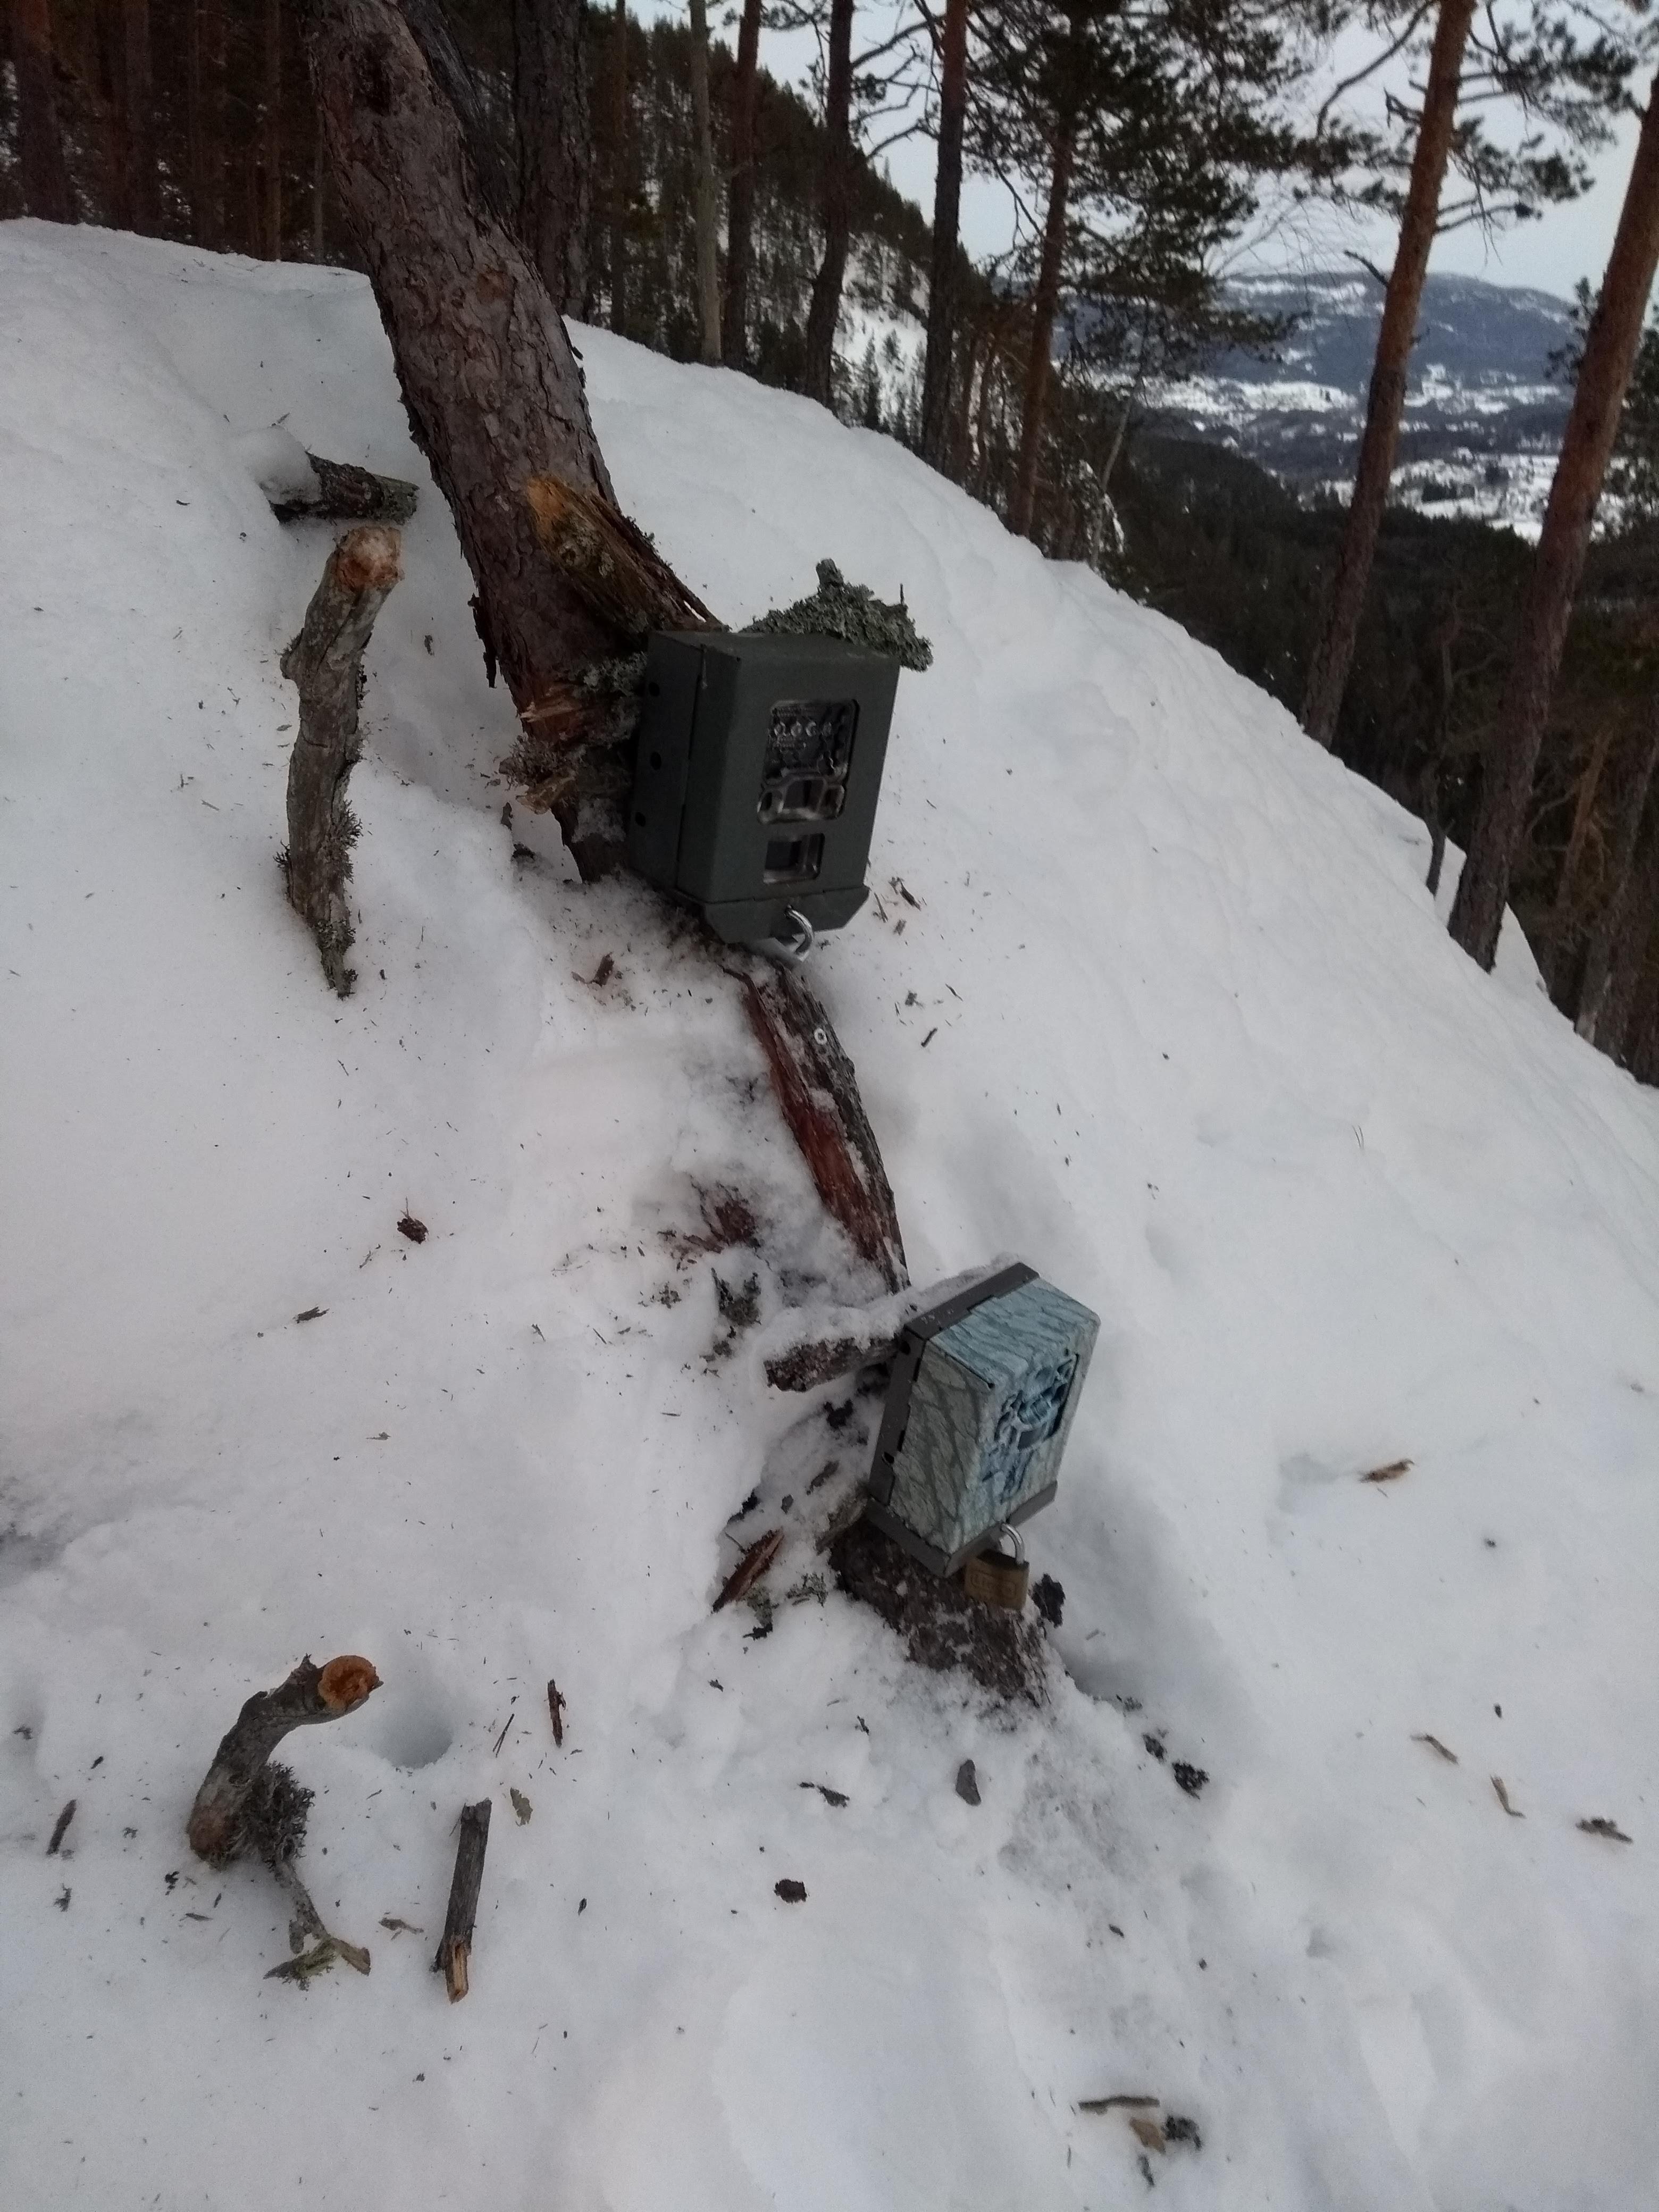
\includegraphics[width=.8\linewidth]{/cam_install_example/IMG_20190212_161615169}
		  \caption{Browning infrared,\\ installed on a fallen tree}
		  	\label{fig:cam_ex_a}
	\end{subfigure}
		\begin{subfigure}{.5\textwidth}
		  \centering
		  	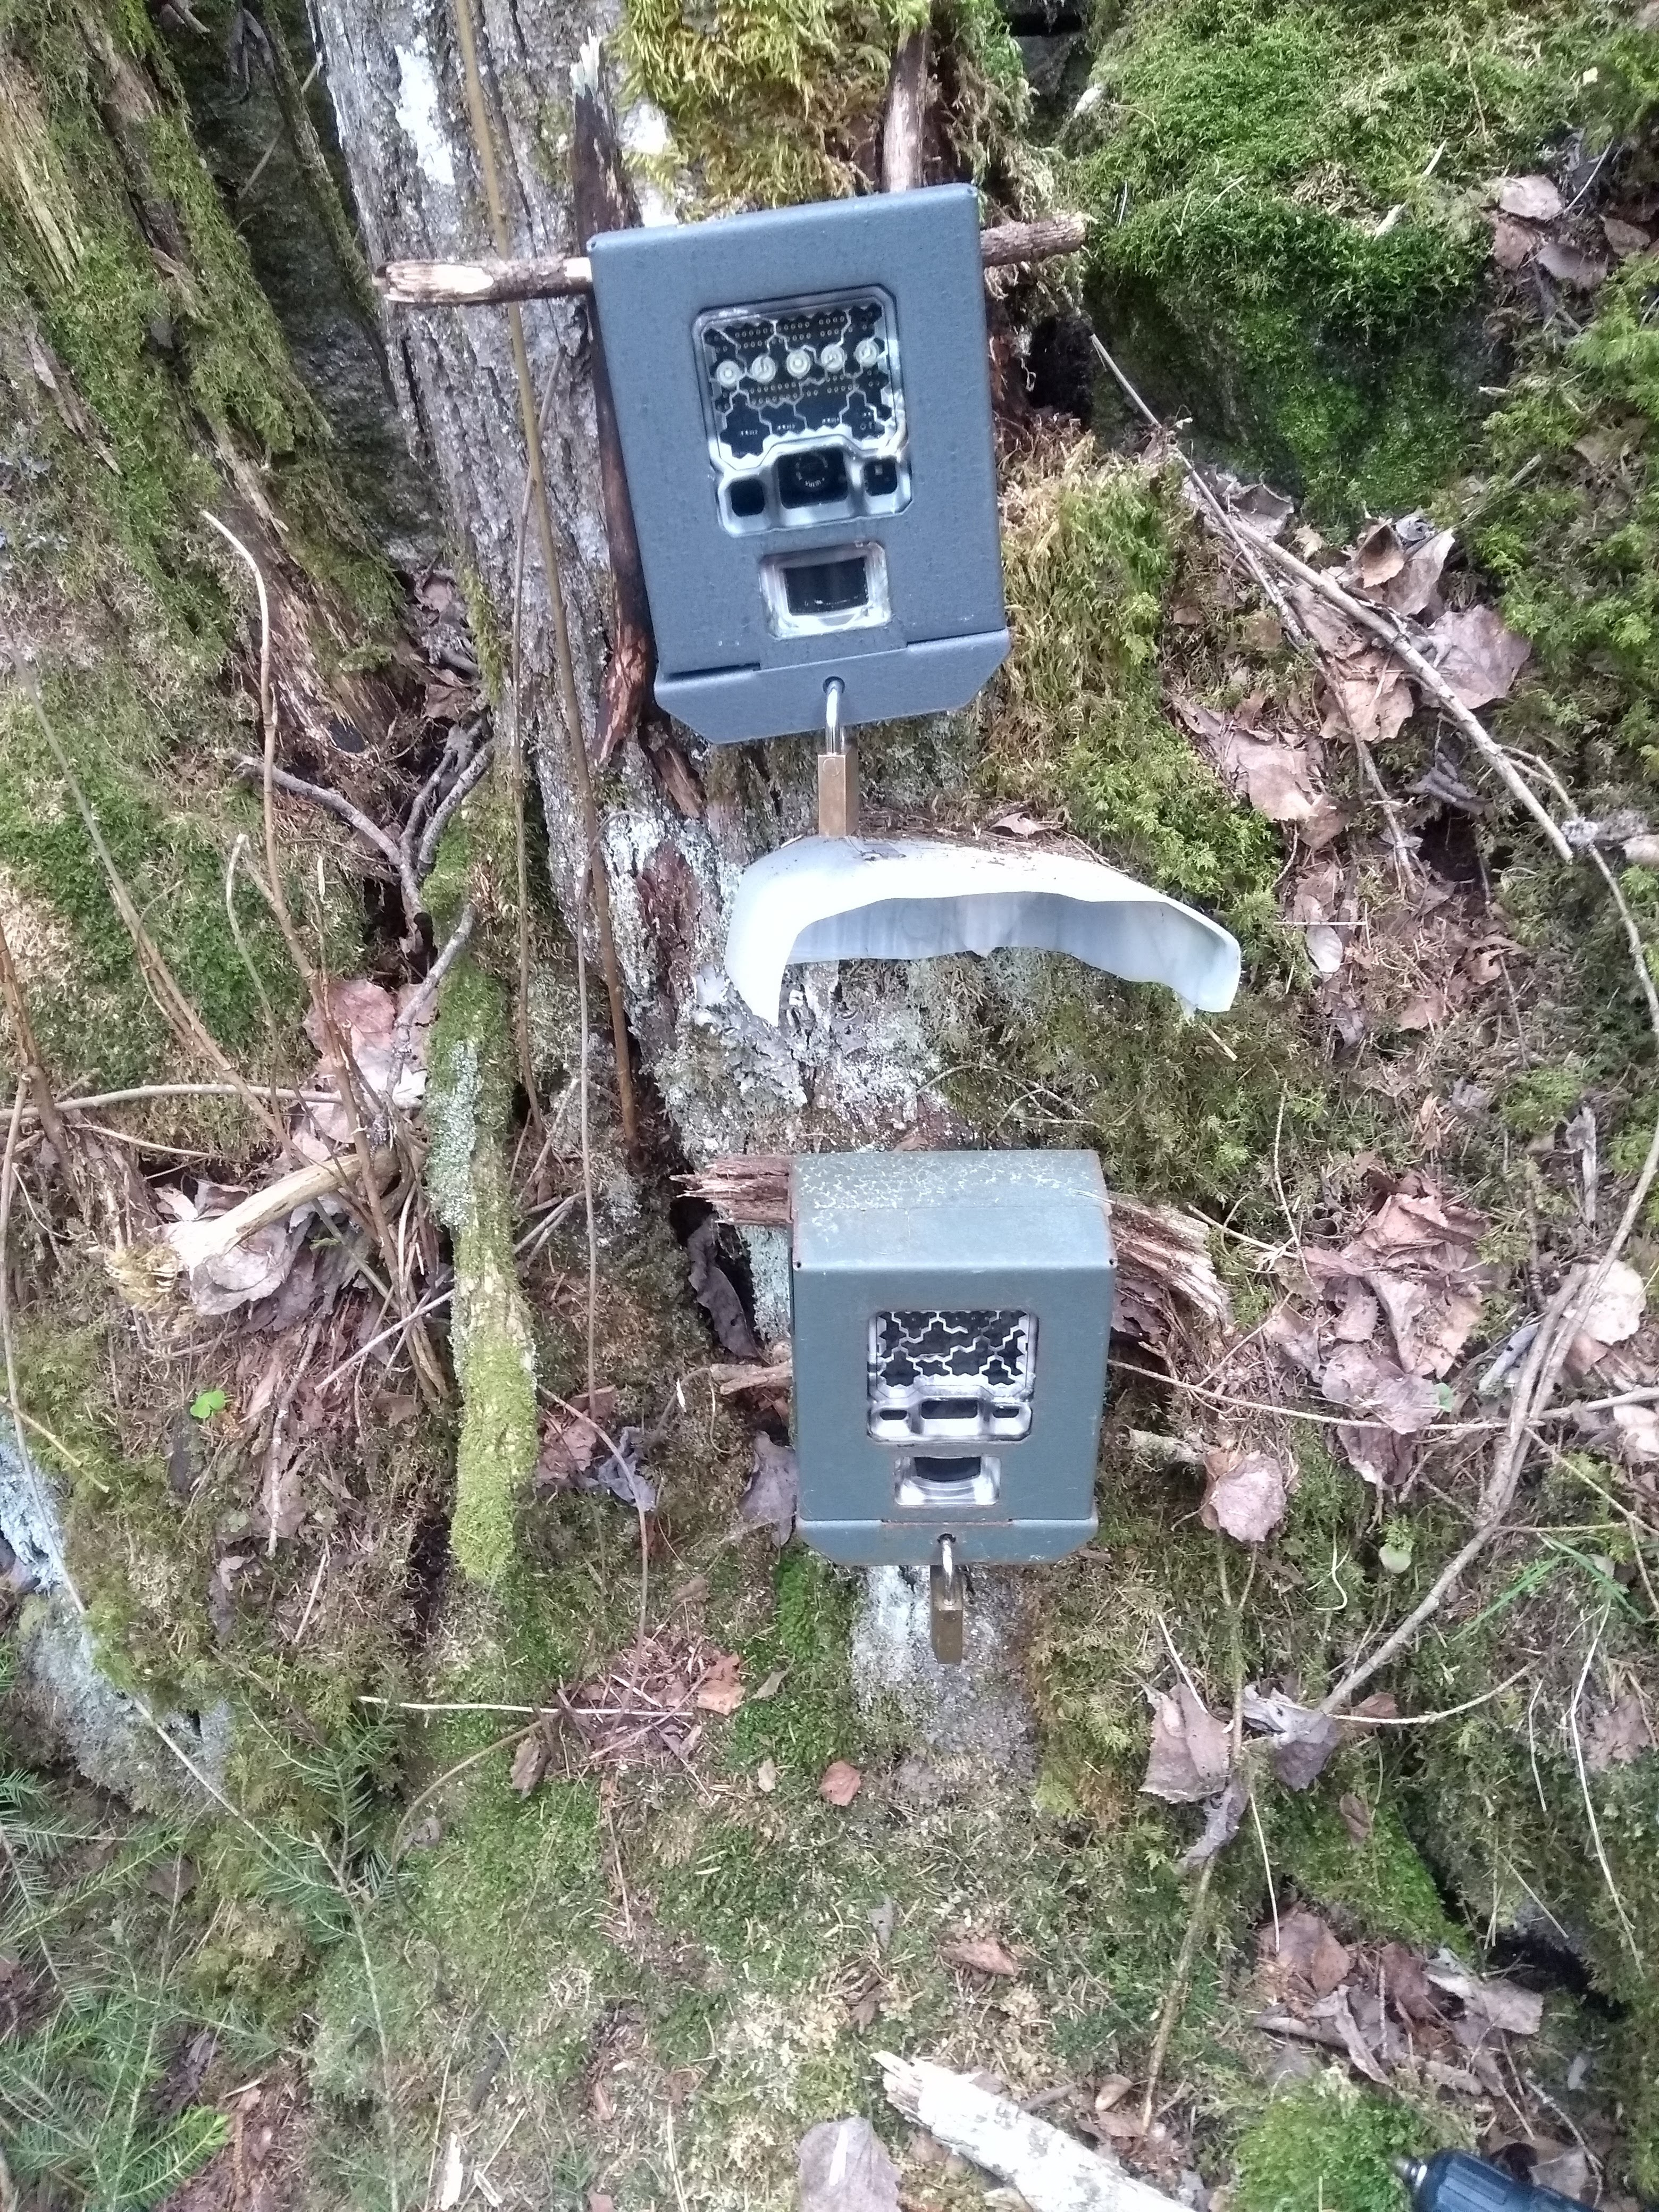
\includegraphics[width=.8\linewidth]{/cam_install_example/IMG_20190515_170952923}
		  \caption{Reconyx infrared,\\ installed with a snow cap}
		  	\label{fig:cam_ex_b}
	\end{subfigure}
		\begin{subfigure}{.5\textwidth}
		  \centering
		  	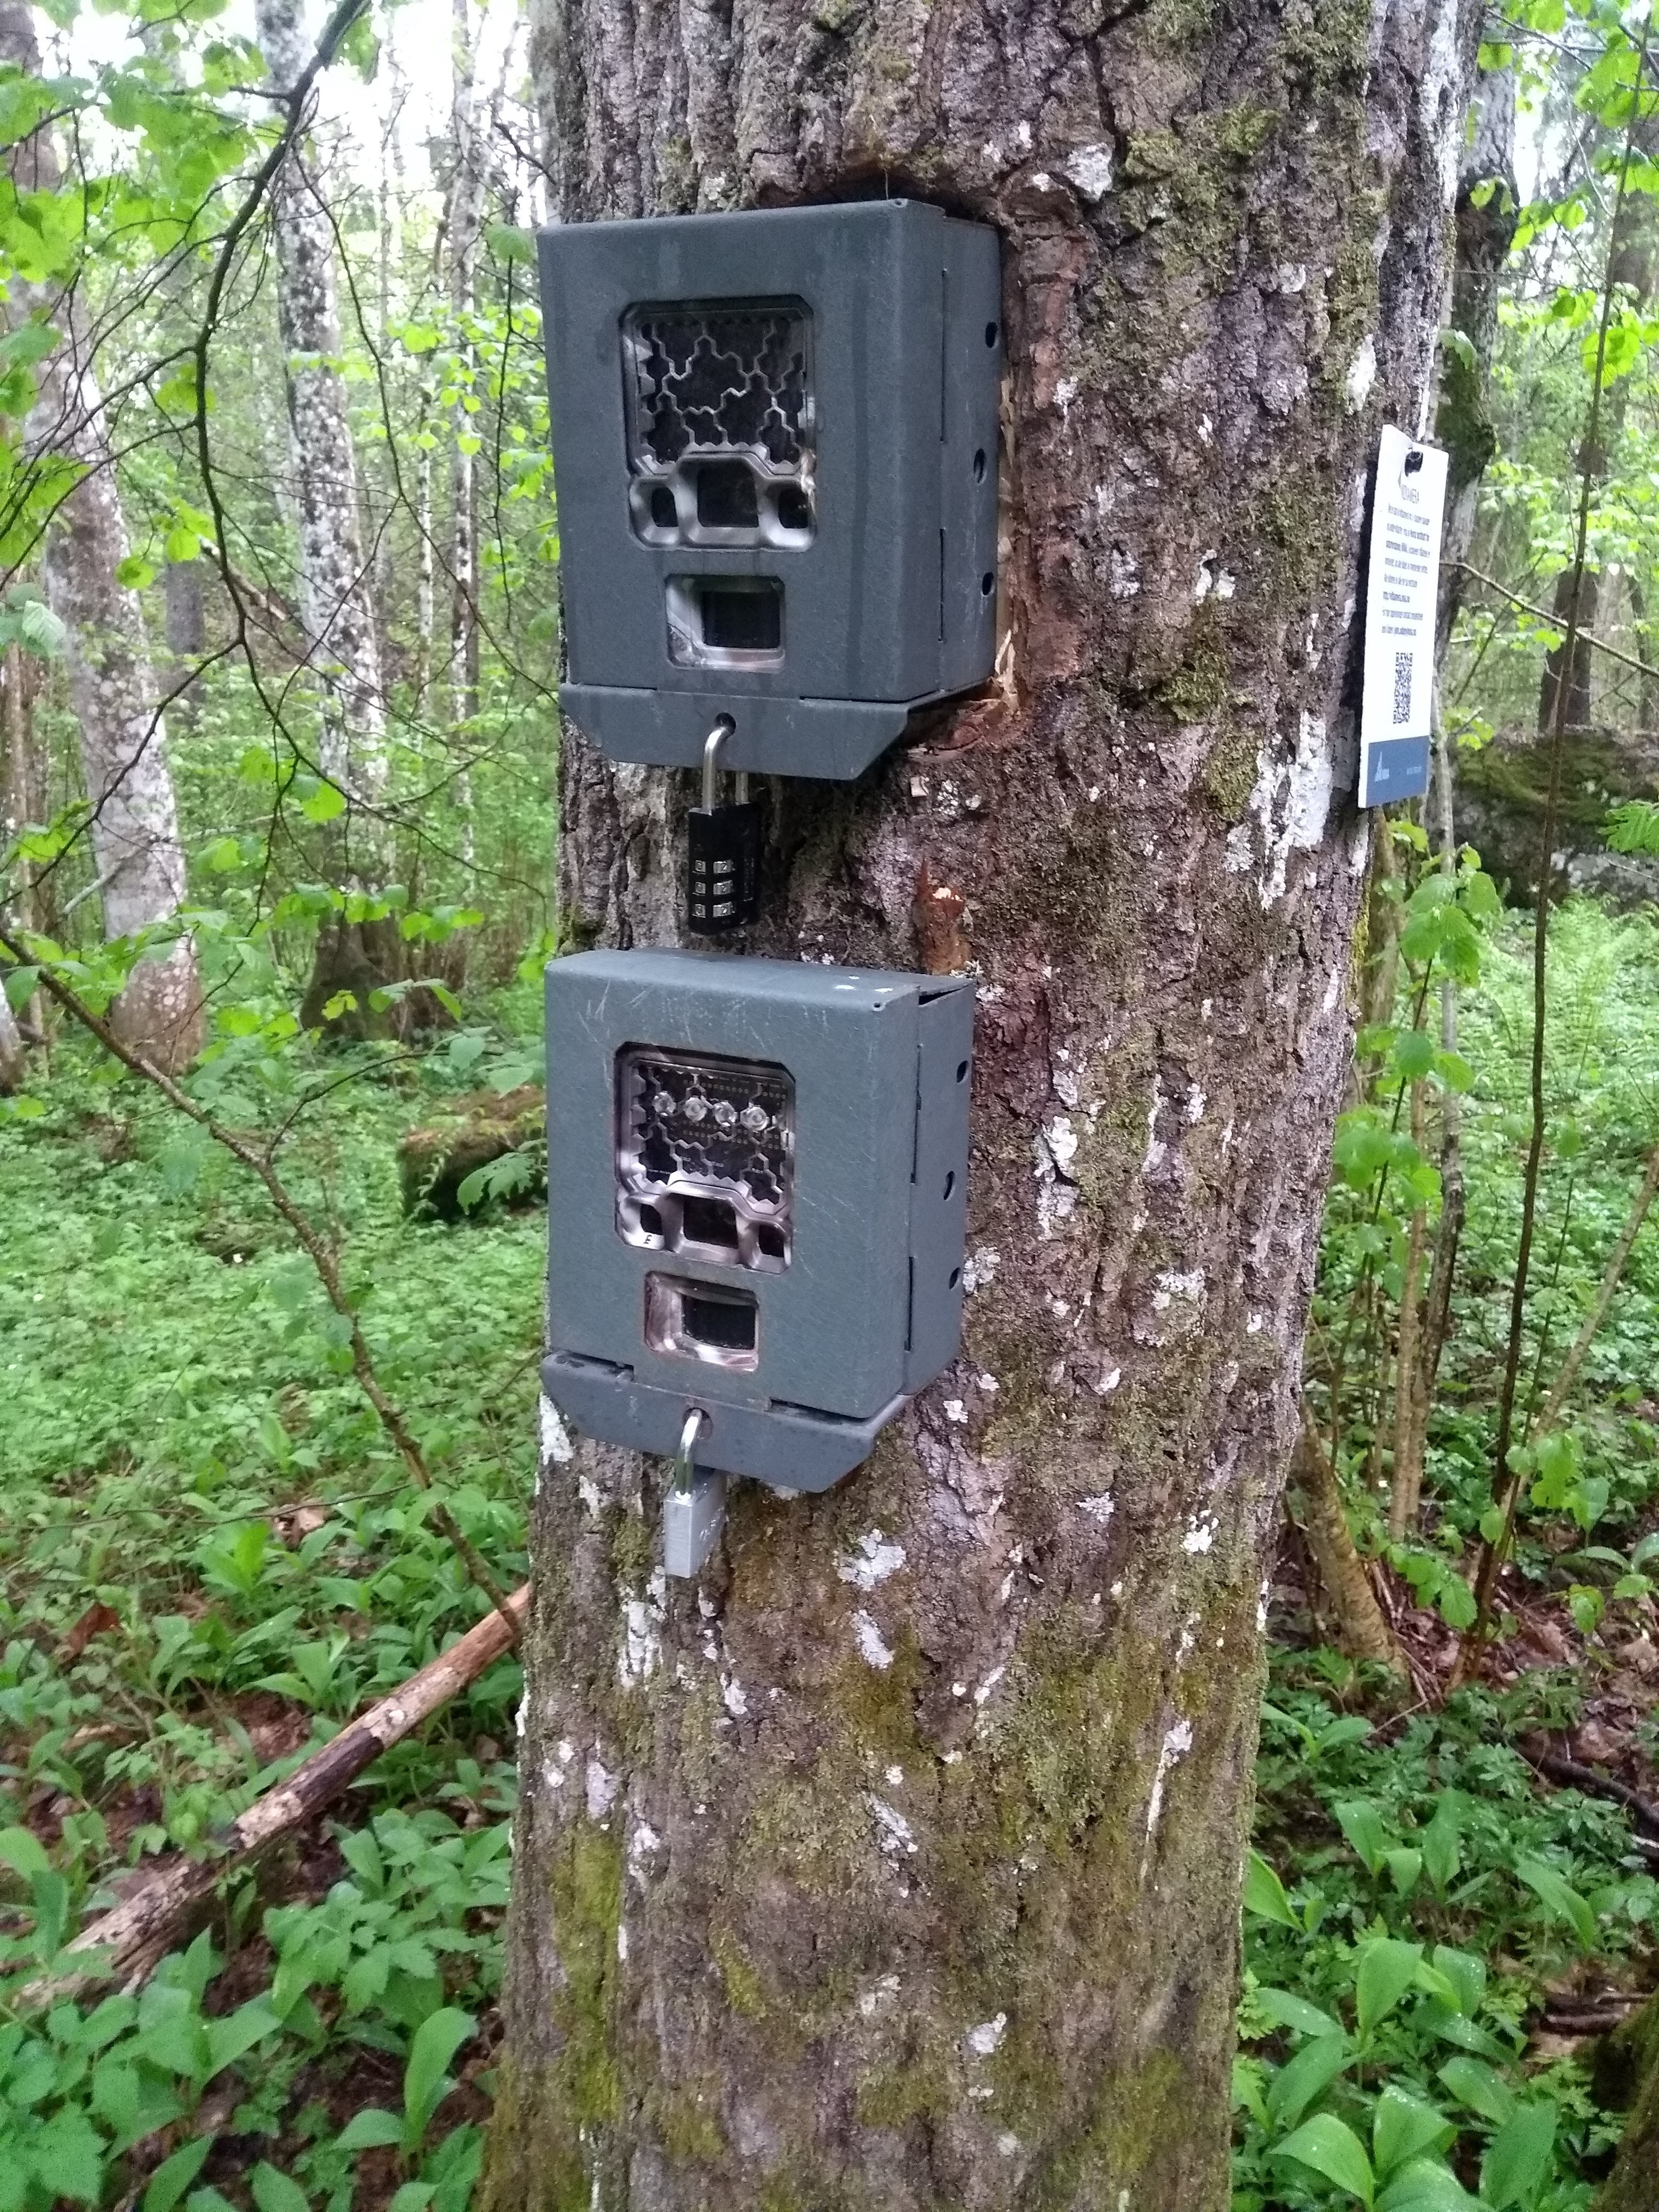
\includegraphics[width=.8\linewidth]{/cam_install_example/IMG_20190521_181329313}
		  \caption{Reconyx infrared above,\\ installed 160 cm above ground level}
		  	\label{fig:cam_ex_c}
	\end{subfigure}
		\begin{subfigure}{.5\textwidth}
		  \centering
		  	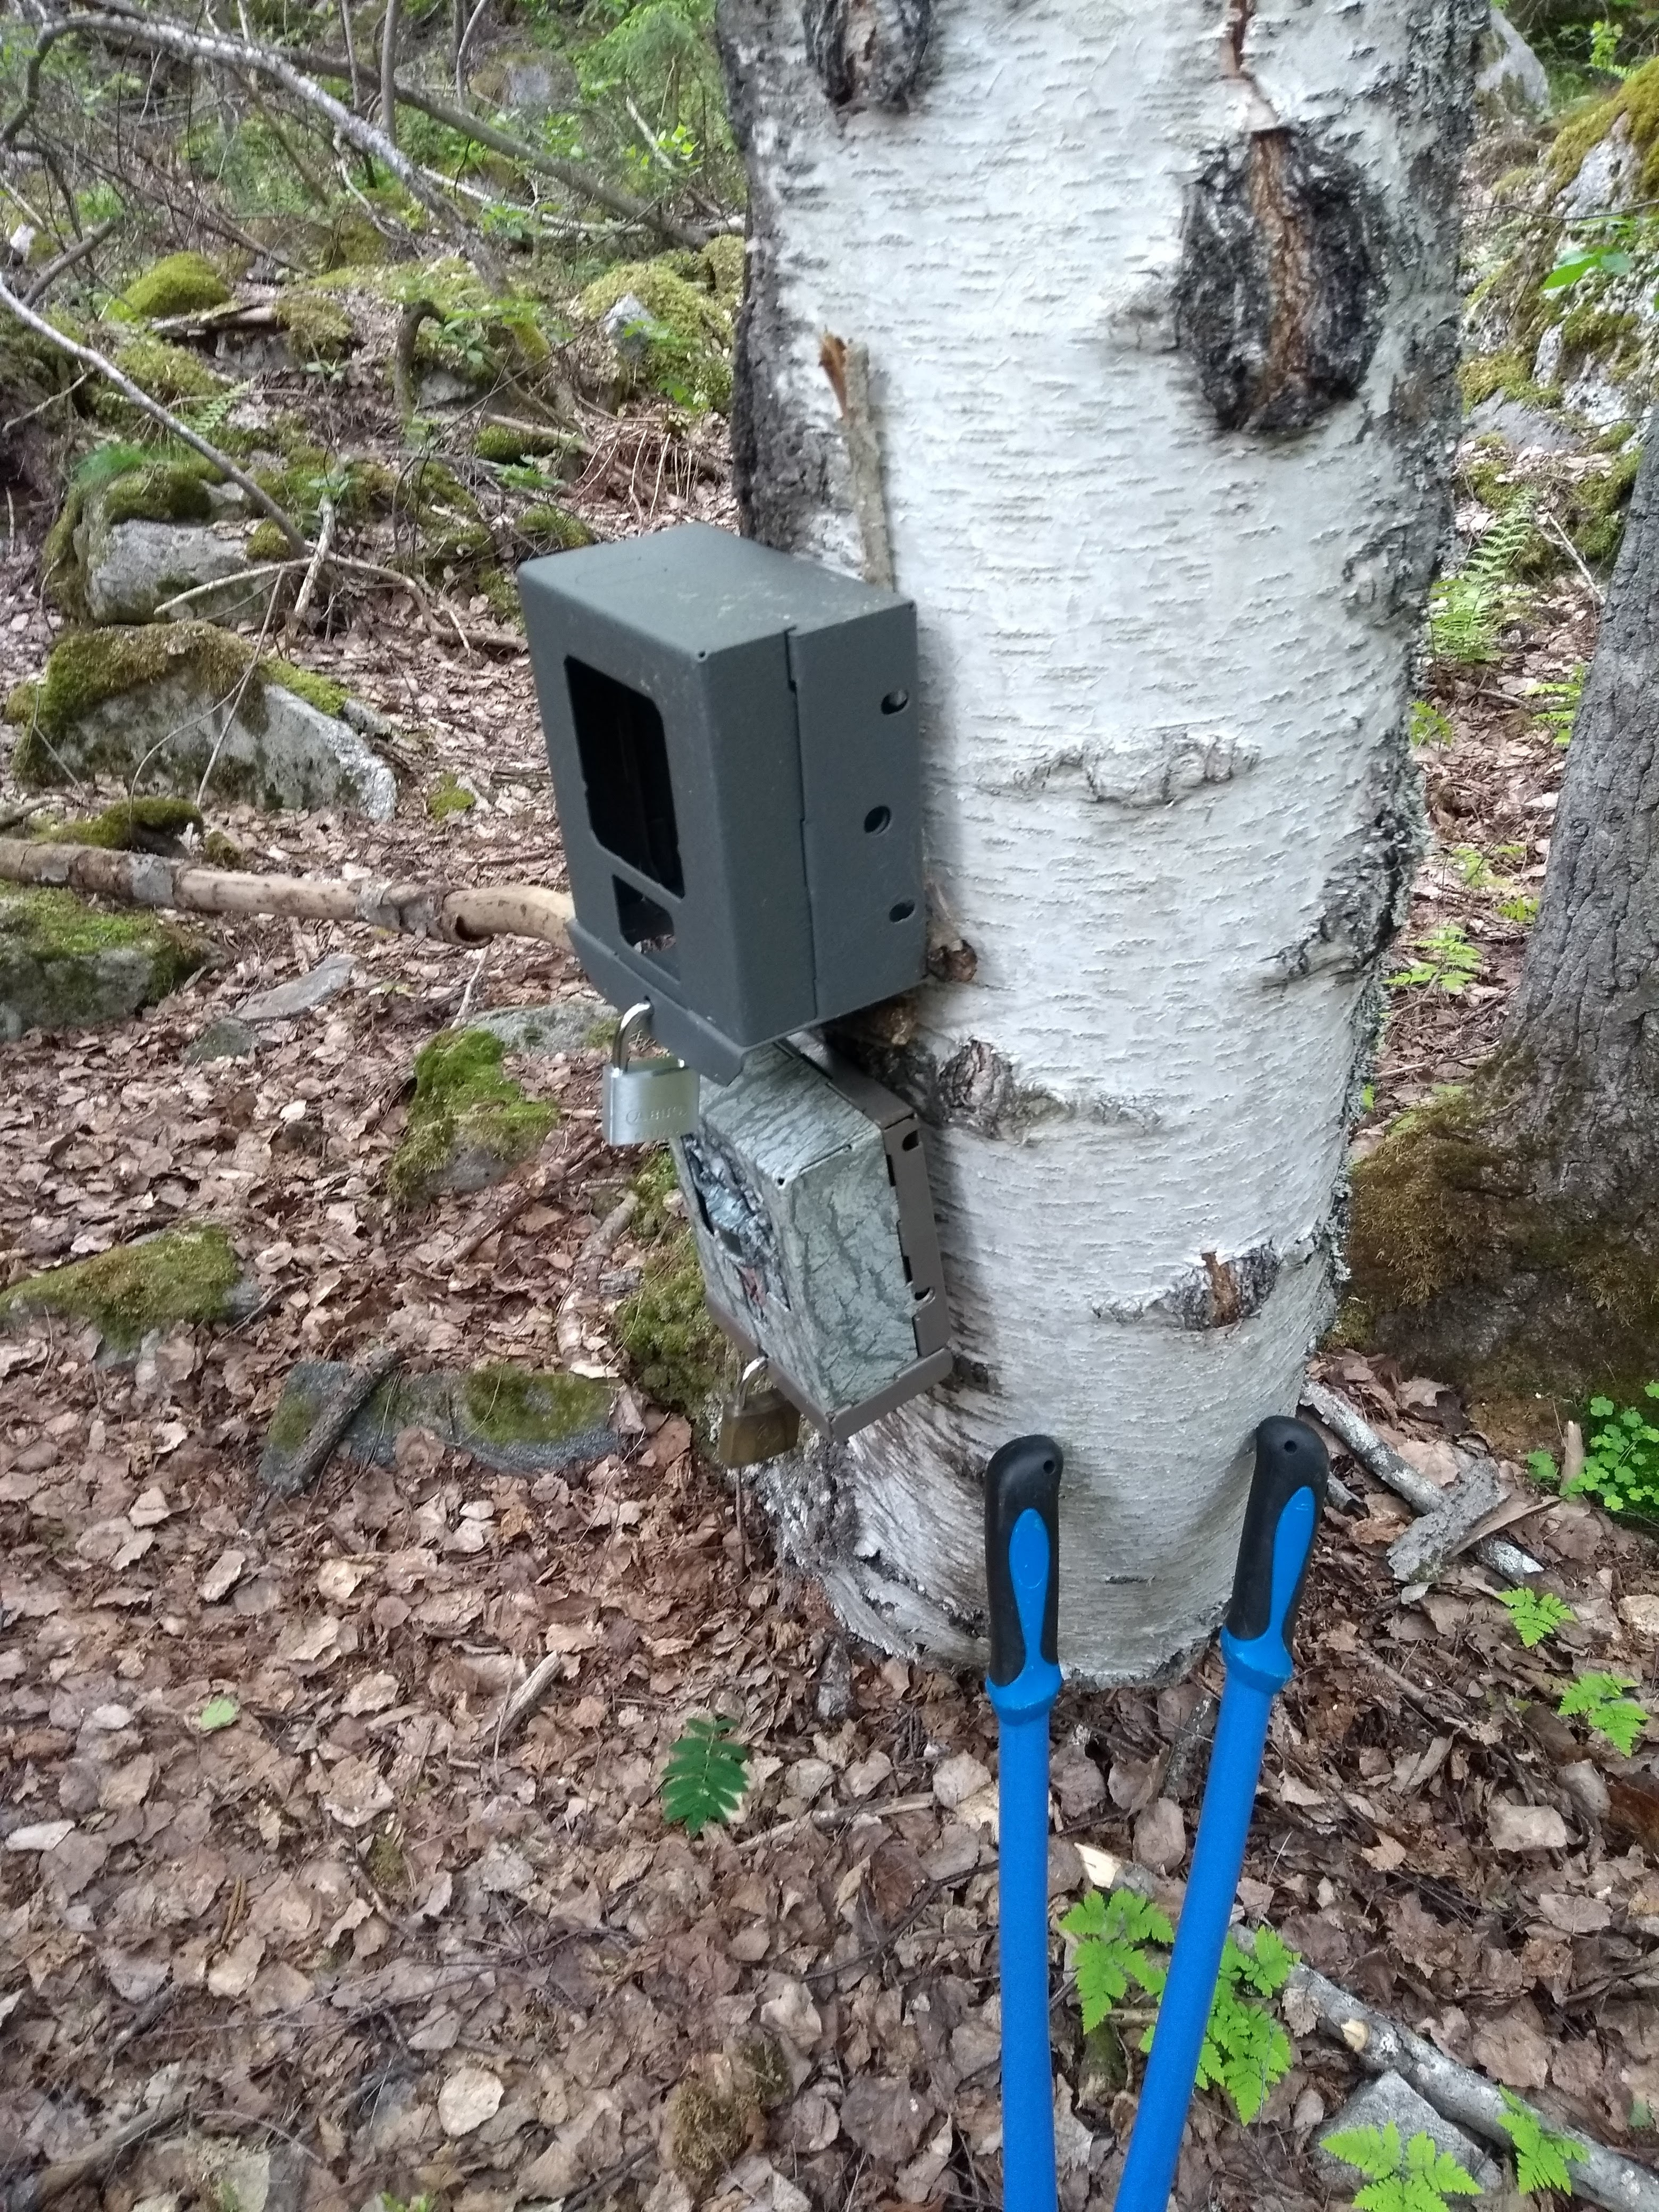
\includegraphics[width=.8\linewidth]{/cam_install_example/IMG_20190529_181049340}
		  \caption{Browning infrared,\\ white LED flash has just been removed}
		  	\label{fig:cam_ex_d}
	\end{subfigure}
		\caption{The preinstalled cameras varied in the way they were set up. Lower cameras with infrared, upper cameras with white LED (except in example c)}
	\label{fig:cam_ex_main}
\end{figure}

%We quantified the degree of consistency in implementing and reporting features of CT protocols and study design that might affect detectability and sampling error (e.g. camera type and settings, spatial and temporal sampling effort, use of attractants; Table S1). These details are fundamental to interpreting results of CT studies and assessing their reliability, repeatability and suitability for broader comparison or synthesis (Meek et al. 2014a)

%TODO Details of camera trap orientation, use of lures, and performance settings are also critical elements of camera trapping methodology. The height in relation to the target, the direction the camera is facing in relation to expected animal travel and path of the sun as well as horizontal and vertical alignment may all influence the results of camera trap studies. Providing clear descriptions of exactly how cameras were placed is fundamental to understanding and interpreting the results of research. (Meek etal 2014)


\section{Data Collection} %TODO  Trenger kilde på AI! 
%The fieldwork was conducted between September 15 and December 20, 2017. In this study, camera traps from the Norwegian Institute for Nature Research (NINA) were used. NINA uses camera traps to monitor the Eurasian lynx in southeastern Norway as part of the SCANDLYNX project (Odden, 2015). SCANDLYNX is a Scandinavian research project on the Eurasian lynx (Odden, 2015; SCANDLYNX, 2017). Camera traps were placed specifically with the goal to photo-capture lynx, and were therefore placed in steep terrain, on ledges or facing the cliff bases, often close to wildlife trails. The cameras were pointing perpendicular to the wildlife trail at locations where a wildlife trail was present. Each camera was mounted on a tree between 0.2 and 1 m above ground

Five different models of RECONYX™ (address: 3828 Creekside Ln, Ste 2, Holmen, WI 54636, USA, www.reconyx.com) cameras were used, 
and one model of BROWNING™ (address: One Browning Place, Morgan, UT 84050, USA, www.browningtrailcameras.com) \ref{tab:cam_mod}.

Reconyx-cameras have been reported of having an average trigger speed of 0.2 seconds, whereas the Browning model was reported an average of 0.7 seconds (Trigger speed shootout, \cite{Trailcampro2014}).


\begin{table}
\caption{\label{tab:cam_mod} Camera models}
\centering

\begin{tabular}{llrrr}
\hline
Producent  & Model name & Flash type & Trigger speed & N \\
\cline{1-2}
\multirow{5}{2cm}{Reconyx HyperFire Series} &
	  HC500 Semi-Covert IR					& IR	& 0.2s &  ? \\
	& HC600 High-Output Covert IR			& Black	& 0.2s &  ? \\
    & PC800 Profoessional Semi-Covert IR 	& IR	& 0.2s &  ? \\
    & PC900 Professional Covert IR 		& Black	& 0.2s &  ? \\
    & PC850 Professional White Flash LED	& White	& 0.2s &  20 \\
\cline{1-2}
Browning  & Spec Ops: Extreme 				& IR	& 0.7s & ~ 24  \\
\hline
\end{tabular}

\end{table}



% [Detection shootout 2017](https://cdn.shopify.com/s/files/1/1065/8354/files/2017_Detection_Shootout_8de2600d-eb3a-42a8-9420-728aae5056e5.pdf?12422955367088316008)

%Reconyx-kameraene har vært programmert til å ha høyest mulig sensitivitet, ta en serie på 3 bilder og ta bildene i raskest mulig rekkefølge («rapidfire»). Neste bildeserie kan startes umid- delbart etter en bildeserie har blitt tatt («no delay»). Vi har i tillegg programmert kameraene til å ta ett bilde hver dag («Time laps»). Dette er viktig for å få tall på nøyaktig hvilke dager kameraene har fungert, eksempelvis når batteri går tomt eller kamera snør ned. Vi har i tillegg valgt høyest mulige bildekvalitet, både med hensyn på antall piksler, lukkertid og rekkevidde på blitsen. Brøste

Cameras were operating 24 hours per day. The RECONYX™ cameras were set to take one time lapse photo per day in order to verify that the cameras had been operational.
The cameras were programmed to have highest possible sensitivity, as described in \cite{Odden2015}. %TODO FINN EIN MÅTE Å SETTE KUN ÅRSTALL I PARANTES
 They were set to take 3 pictures per series, as fast as possible using \emph{rapidfire}, and retrigger immediately using \emph{no delay}.
At the start of the study, I adjusted the BROWNING™ camera settings from 3 to 8 photos per trigger, in order to gather more data on behavioural responses to the white LED flash stimuli. 
However, behavioural responses are beyond the scope of this study. %TODO  Atle: Then why did you do it?


Unfortunately, with such data heavy settings, memory cards are more vulnerable to filling up before being collected, in areas with sheep and cattle, or when cameras get triggered by grass or branches blowing in the wind. Therefore, the BROWNING™ cameras, which also happen to be the northernmost cameras, tended to have more gaps of inoperable days. %Må reinskrivast/skrivast betre

Whenever I noticed vegetation blocking the view of the camera, or excessively triggering it, I removed the vegetation.

%difference between the two camera types*** 
% Assumptions: chance of detection & sp validation BROWNING > RECONYX, operational days BROWNING < RECONYX








\section{Data processing} %TODO
All SD cards were delivered to NINA for data collection. Firstly, a facial recognition algorithm (FRA)  is used to sort all the pictures. %artificial intelligence software (AI)
Afterwards, a human sorter checks the softwares' output, confirming all the correct decisions (i.e. species detections) and correcting all the wrong ones.
The goal is to fully automate this process, which is a request from The Norwegian Data Protection Authority (DPA) in relation to usage of cameras in densely crowded areas (e.g. parks).
As per the four eyes principle, the detection rate of photographed species has gone up as a result of the FRA (pers.comm. John Odden). 

%Nei, vi har ikke publisert artikkel på gjenkjenningsalgoritmen. Du har jo vært med på prosessen sjøl, så jeg veit ikke om du egentlig trenger referanse her, men du kan sette inn John O som pers med og merke det, så kan han eller jeg endre det slik vi mener det bør være når vi leser gjennom oppgava di..


The output I got as a result, was a data frame containing a time stamp for every shutter activity, %kvar gong eit bilde blei tatt
including all meta data from the camera, coupled with predicted species (FRA output, with a confidence number), verified species (by human sorters), number of animals and distance from camera. The time stamps from the white flash cameras were used to verify whether an animal was in fact flashed or not, which I then used as my main predictor in the modelling. 
%Describing in brief how coding is undertaken is useful for readers to understand the methods used in relation to the results.(Meek etal 2014)


I defined one event as any 1 species passing with a buffer time of 5 min before or after %TODO  Må bestemme lengde på intervall, og formulere betre


The true number of active camera days are confounded by the inconvenient lack of time lapse photos from the Browning cameras. To approach the true number of active days, I assumed all Browning cameras to be functional every day, unless the camera was inactive when I visited it. In that case, I considered the camera inactive since the day of its last photo.



%*************************************************************
%
%Hypothesis 1: Usage of white LED flash will stress one or more species in general, and therefore lower the detection rate of the stressed species. The effect will likely vary in extent between species.
%
%*************************************************************
%
%Hypothesis 2: The effect of the white LED will correlate with urbanisation-factors, as individuals that live closer to urban areas are habituated to Artificial Light At Night (ALAN), and thus will have a weaker response to the white LED
%
%


\section{Statistical analysis} %This is a reference to the session info appendix \ref{app:sessinfo}

To test for effects of the white LED flash I used the R programming language (\cite{RCoreTeam2020}), in the RStudio IDE (\cite{RStudioTeam2020a}), adopting large parts of the tidyverse framework along the way (\cite{tidyverse}). Session info in appendix \ref{app:sessinfo}.

\subsection*{Multiple hypothesis testing}
%Alpha defined in holm and in shaffer
When testing multiple groups for significance, the false positive rate will inevitably go up. 
By chance, if I tested 20 groups where the $H_{0}$ were true, an $\alpha = 0.05$ 
($ =  \frac{1}{20} $) 
would deem at least one of the groups to be significantly different, thus rejecting the $H_{0}$ on false terms (ie. commiting a type 1 error).
Therefore, when testing six species, I should demand stronger evidence to reject the null hypothesis.
The Bonferroni correction (\cite{Holm1979}) is straight forward, multiplying each p-value by the number of comparisons, or in other words dividing the $\alpha$ by the number of comparisons. This highly diminishes the chance of commiting type 1 errors, but unfortunately increases the chance of type 2 errors (failing to reject a false null hypothesis) \cite{Shaffer1995}. 
In my case, using the Bonferroni correction would result in:

 $$ \alpha = \frac{0.05}{ 6 \mbox{\ species} } = 0.0083 \mbox{\ per species} $$ 


A less conservative method is the sequentially rejective Bonferroni test (\cite{Holm1979}), often called Holm method, which is a modification of the Bonferroni correction. Here, the most significant test is given the Bonferroni correction ($\alpha /n$ tests).
Then, the second most significant test gets an $\alpha / n - 1$, or, a slightly larger alpha.
Continuing untill the least significant test gets an $\alpha / 1$ (i.e. retains the original $\alpha = .05$). In my case, using the Holm method results in:

 $$ \frac{\alpha}{6},\ \frac{\alpha}{6-1},\ ...,\ \frac{\alpha}{1} $$


	\subsection*{Hypothesis 1}

To test $H_{1}$ I looked for differences in mean detection rate per day, using Generalised Linear Mixed Models (GLMM) with the R package lme4 (\cite{lme4}). White LED present/absent was the predictor, while location ID and month was used as random factors, to control for underlying differences between sites, and seasonal changes.



In addition, I used a Cox proportional hazards regression model (CPH model) (Cox, 1972), as a time to event analysis. 
Also called Survival analysis, the model compares groups' risk of experiencing an event (the \emph{hazard ratio} between the groups) , and was first developed for use in medicinal studies (e.g. cancer risk studies).

I used the CPH model to elaborate on the effect of the white LED by checking whether \emph{confirmed} events of a flashed species affected the time untill said species' \emph{re}detection. The coxme function from the coxme package (\cite{coxme-package}) was used to include random effect arguments.


	\subsection*{Hypothesis 2}

If the $H_{0}$ was rejected for a species, I tested the $H_{2}$.
To do that, I performed a new Cox PH, without the random effects, and looked for an interaction between the flashed-variable, and a spatial covariate for distance to nearest ALAN 
(data from FKB). %TODO 
This time, I used the coxph function from R package Survival (\cite{survival-package}).


	\subsection*{P-tests and assumptions}

For the GLMM, I used a XX as p-test 
For the Cox model, I used the Wald test as the significance test, with xyz distribution over df degrees of freedom. osvosv. 


%Attention devoted to model assumptions! Viktig i Burton 2015
The XX was used to check assumptions for GLMM  %TODO assumptions of glmm

The Schoenfeld test was used to check for the survival model's assumption of proportional hazards. 


	\subsection*{GLMM}
GLMM model was fitted to identify if flash had an effect on detection rates of different species. A mixed effect model was required to include both fixed and random effects.
*Generalised model was needed because of the usage of both continuous and categorical predictors. (ACTUALLY DON'T KNOW!)


--------

"Note that the random estimate means are closer to the overall mean, reflecting that the model assumes each subject's mean is closer to the overall average than it actually is --- a fundamental "assumption" of a multilevel model."  - Pierce Edmiston 2014 (Visualizing lmer model random effects, November 1 2014, accessed 16.02.2021) 

--------


	\subsection*{Cox Proportional Hazards}
What I am in truth testing is each camera's chance of contracting a roe deer disease, or fox disease, and how that chance changes when "treated" with a white LED flash.
	\subsection*{P-tests and assumptions}

%\subsection{AIC old}

%If you are using AIC model selection in your research, you can state this in your methods section. Report that you used AIC model selection, briefly explain the best-fit model you found, and state the AIC weight of the model.

%For each species, I used the Akaike Information Criterion (AIC) to select the best models excluding the flashed-predictor.
%Then, I added the flashed-predictor to each species top model, to see whether this effect could account for any remaining variation.
%
%
%Example: 
%
%We used AIC model selection to distinguish among a set of possible models describing the relationship between age, sex, sweetened beverage consumption, and body mass index.
%The best-fit model, carrying 97\% of the cumulative model weight, included every parameter with no interaction effects.

%After finding the best-fit model you can go ahead and run the model and evaluate the results. The output of your model evaluation can be reported in the results section of your paper.




% -- results --
\chapter{Results}
%\subsection{General results}
%
%After excluding faulty cameras we had TK cameras in total, 19 in the Control-group and 33 in the experiment group.
%A total of TK photos were taken, of whom TK contained photos of the species I've focused on in my study. Check table for more details.
%
%The species I've focused on was mainly night-active as displayed in the density plots \ref{fig:overlap}, (with the exception of squirrel). In other words, all of them experienced a white LED flash during night hours.
%(Caption: Figure is split up in periods with and without white LED flash. Night activity in the dashed curve highlights the times the species would have experienced the flash. "Carpet"-below the curves signifies datapoints of each "group".
%



%\section{All species} %AMkomm: Title needs to say something more

As the control-group (Intercept in table \ref{tab:param}) stayed unchanged through the whole study period, and was visited less than the other cameras, I expected there to be no trend over time (i.e. time.deploy $\approx 0$ in table \ref{tab:param}).
Any fluctuations in detection rates due to weekly (and ultimately seasonal) changes should be controlled for by the random effect-term for week of the year, leaving the control group as a representation of the baseline detection rate.
This held true for all the species in my analysis.

In general, the control-group had lower detection rates than the two treatment groups for all species (see table \ref{tab:param}).
However, for most species, the slopes of IR and LED are completely covered by the Control-group's confidence interval (CI), meaning that the differences are non-significant.


If there were any effect of the LED, the IR period should show a regression to the norm, ie. counteracting the effect of the LED.
Thus, if the LED had a negative slope along the time axis, the IR should have a positive slope.
Further, their respective main effects (ie. when time since deployment = 0) should correspond somewhat to the other factor's simple effect of when time since deployment is at maximum value (84 days).
Still, as time since deployment = 0 corresponds to the day of my visitation, my presence could skew that pattern to some extent.

The main effect of LED was positive for most species, although none responded significantly (table \ref{tab:param}).

\begin{table}[ht]
\caption[Model parameters]
{\label{tab:param} Model parameters \par \small Results of generalised linear mixed effect models on detection rate of species at 56 different locations in south-eastern Norway, with three different treatment levels; periods from sites unchanged through the the whole study period (Intercept), period with only IR camera (IR) and period with additional white LED camera (LED). Random effects are location ID and week of year. %Standardised parameters were obtained by fitting the model on a standardised version of the dataset.
95\% Confidence Intervals and p-values were computed using the Wald approximation.}

% latex table generated in R 4.0.4 by xtable 1.8-4 package
% Fri Mar 26 20:35:32 2021
\centering
{\tiny\renewcommand{\arraystretch}{.8}
	\resizebox{!}{.35\paperheight}{%
		\begin{tabular}[c]{llrlcrrr}
  \toprule
Species & Parameter & Coefficient & SE & 95\% CI & z & p & SGPV \\ 
\midrule
Roe deer & Intercept & -2.85 & 0.38 & (-3.58, -2.11) & -7.57 & $<$ .001 & 0.00 \\ 
& Time & -0.05 & 0.02 & (-0.09, -0.01) & -2.24 & \textbf{0.025}  & \textit{1.00} \\ 
& IR & -0.26 & 0.44 & (-1.12,  0.60) & -0.59 & 0.557  & 0.14 \\ 
& wLED & -0.13 & 0.44 & (-0.99,  0.73) & -0.30 & 0.761  & 0.14 \\ 
& Time * IR & 0.02 & 0.03 & (-0.04,  0.08) & 0.71 & 0.476  & \textit{1.00} \\ 
& Time * wLED & $<$ 0.01 & 0.03 & (-0.05,  0.06) & 0.12 & 0.901  & \textit{1.00} \\ 
\midrule
Moose & Intercept & -4.15 & 0.30 & (-4.75, -3.56) & -13.75 & $<$ .001 & 0.00 \\ 
& Time & $<$ 0.01 & 0.05 & (-0.08,  0.10) & 0.14 & 0.890  & \textit{1.00} \\ 
& IR & 		-0.08 & 0.35 & (-0.77,  0.60) & -0.23 & 0.814  & 0.17 \\ 
& wLED & 	 0.30 & 0.34 & (-0.36,  0.97) & 0.89 & 0.373  & 0.18 \\ 
& Time * IR & 0.05 & 0.06 & (-0.06,  0.17) & 0.86 & 0.389  & 0.75 \\ 
& Time * wLED & $<$ 0.01 & 0.06 & (-0.12,  0.10) & -0.12 & 0.902  & \textit{1.00} \\ 
\midrule
Red deer & Intercept & -3.89 & 0.41 & (-4.69, -3.09) & -9.55 & $<$ .001 & 0.00 \\ 
& Time & -0.09 & 0.06 & (-0.21,  0.02) & -1.63 & 0.104  & 0.53 \\ 
& IR & $<$ 0.01 & 0.50 & (-0.99,  0.97) & -0.02 & 0.984  & 0.12 \\ 
& wLED & -0.69 & 0.53 & (-1.72,  0.35) & -1.30 & 0.192  & 0.12 \\ 
& Time * IR & 0.06 & 0.08 & (-0.09,  0.21) & 0.81 & 0.421  & 0.65 \\ 
& Time * wLED & 0.23 & 0.08 & ( 0.08,  0.38) & 2.96 & \textbf{0.003}  & 0.00 \\ 
\midrule
Badger & Intercept & -4.49 & 0.37 & (-5.22, -3.76) & -12.12 & $<$ .001 & 0.00 \\ 
& Time & 0.06 & 0.03 & ( 0.00,  0.13) & 1.85 & 0.064  & 0.82 \\ 
& IR & 0.17 & 0.39 & (-0.59,  0.93) & 0.44 & 0.657  & 0.16 \\ 
& wLED & 0.24 & 0.38 & (-0.51,  0.99) & 0.64 & 0.523  & 0.16 \\ 
& Time * IR & 0.01 & 0.04 & (-0.07,  0.09) & 0.27 & 0.784  & \textit{1.00} \\ 
& Time * wLED & $<$ 0.01 & 0.04 & (-0.07,  0.08) & 0.11 & 0.914  & \textit{1.00} \\ 
\midrule
Pine Marten & Intercept & -5.95 & 0.54 & (-7.02, -4.89) & -10.95 & $<$ .001 & 0.00 \\ 
& Time & 0.09 & 0.09 & (-0.09,  0.28) & 0.97 & 0.331  & 0.52 \\ 
& IR & 1.69 & 0.58 & ( 0.55,  2.82) & 2.92 & \textbf{0.004}  & 0.00 \\ 
& wLED & 0.76 & 0.61 & (-0.43,  1.95) & 1.25 & 0.210  & 0.10 \\ 
& Time * IR & -0.11 & 0.11 & (-0.32,  0.09) & -1.07 & 0.286  & 0.46 \\ 
& Time * wLED & 0.03 & 0.11 & (-0.18,  0.24) & 0.30 & 0.768  & 0.56 \\ 
\midrule
Red fox & Intercept & -3.44 & 0.26 & (-3.94, -2.94) & -13.40 & $<$ .001 & 0.00 \\ 
& Time & $<$ 0.01 & 0.03 & (-0.06,  0.05) & -0.02 & 0.985  & \textit{1.00} \\ 
& IR & 0.03 & 0.32 & (-0.59,  0.65) & 0.09 & 0.926  & 0.19 \\ 
& wLED & 0.18 & 0.31 & (-0.44,  0.79) & 0.56 & 0.574  & 0.19 \\ 
& Time * IR & $<$ 0.01 & 0.04 & (-0.08,  0.07) & -0.06 & 0.949  & \textit{1.00} \\ 
& Time * wLED & -0.01 & 0.04 & (-0.08,  0.06) & -0.30 & 0.763  & \textit{1.00} \\ 
\midrule
Lynx & Intercept & -4.82 & 0.58 & (-5.96, -3.67) & -8.24 & $<$ .001 & 0.00 \\ 
& Time & -0.22 & 0.14 & (-0.49,  0.05) & -1.58 & 0.113  & 0.24 \\ 
& IR & -0.20 & 0.72 & (-1.61,  1.21) & -0.28 & 0.781  & 0.08 \\ 
& wLED & 0.15 & 0.72 & (-1.26,  1.55) & 0.20 & 0.839  & 0.08 \\ 
& Time * IR & 0.25 & 0.16 & (-0.07,  0.57) & 1.53 & 0.127  & 0.22 \\ 
& Time * wLED & 0.26 & 0.16 & (-0.06,  0.58) & 1.59 & 0.112  & 0.20 \\ 
\midrule
Hare & Intercept & -3.91 & 0.36 & (-4.61, -3.21) & -10.94 & $<$ .001 & 0.00 \\ 
& Time & 0.04 & 0.03 & (-0.03,  0.10) & 1.12 & 0.263  & \textit{1.00} \\ 
& IR & 0.38 & 0.42 & (-0.44,  1.21) & 0.91 & 0.363  & 0.14 \\ 
& wLED & 0.25 & 0.42 & (-0.58,  1.08) & 0.59 & 0.555  & 0.14 \\ 
& Time * IR & -0.05 & 0.04 & (-0.13,  0.03) & -1.26 & 0.209  & 0.88 \\ 
& Time * wLED & $<$ 0.01 & 0.04 & (-0.08,  0.08) & 0.03 & 0.975  & \textit{1.00} \\ 
\midrule
Red squirrel & Intercept & -4.82 & 0.41 & (-5.63, -4.00) & -11.63 & $<$ .001 & 0.00 \\ 
& Time & 0.08 & 0.05 & (-0.01,  0.18) & 1.67 & 0.095  & 0.62 \\ 
& IR & 0.91 & 0.47 & (-0.02,  1.83) & 1.93 & 0.054  & 0.00 \\ 
& wLED & 0.61 & 0.48 & (-0.32,  1.54) & 1.28 & 0.201  & 0.13 \\ 
& Time * IR & -0.17 & 0.06 & (-0.29, -0.05) & -2.85 & \textbf{0.004}  & 0.13 \\ 
& Time * wLED & -0.02 & 0.06 & (-0.13,  0.10) & -0.29 & 0.771  & 0.92 \\ 
   \bottomrule
\end{tabular}}}

	%Caption outside the .tex-file or else it would be deleted every time I update the parameter-table

\end{table} % må inn og fjerne end{table} (vertfall \begin{table}) kvar gong tabellen oppdaterest!

 
%

\begin{figure}
		\begin{subfigure}{.5\textwidth}
		  \centering
		  	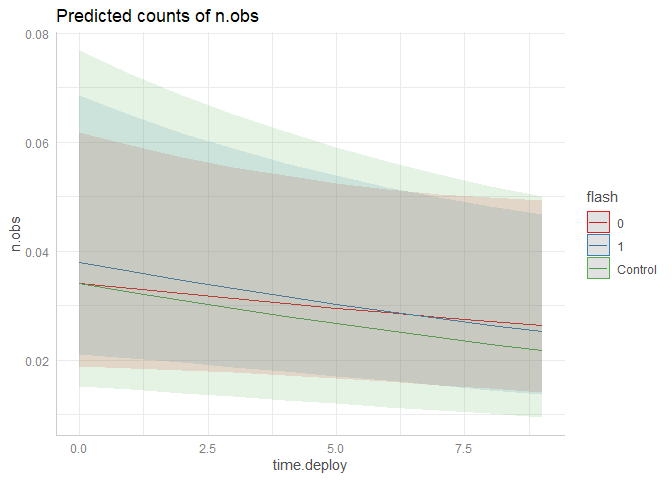
\includegraphics[width=.8\linewidth]{../R/glmm_sp_files/figure-gfm/raadyr-C-report-1.png}
		  \caption{Roe deer}
		  	\label{fig:glmm_raa}
	\end{subfigure}
		\begin{subfigure}{.5\textwidth}
		  \centering
		  	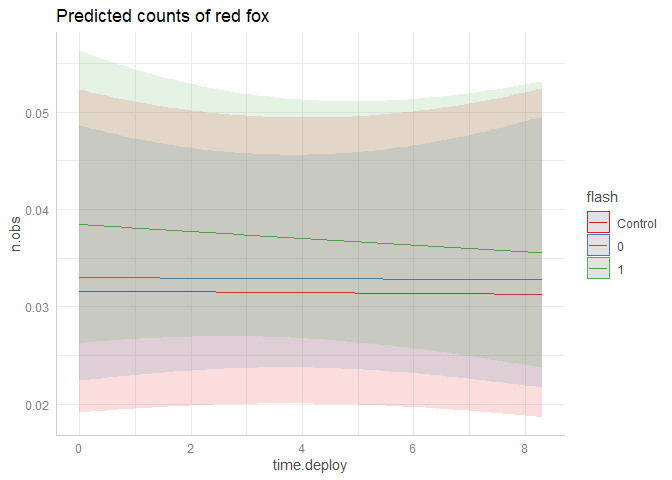
\includegraphics[width=.8\linewidth]{../R/glmm_sp_files/figure-gfm/rev-report-1.png}
		  \caption{Red fox}
		  	\label{fig:glmm_rev}
	\end{subfigure}
		\begin{subfigure}{.5\textwidth}
		  \centering
		  	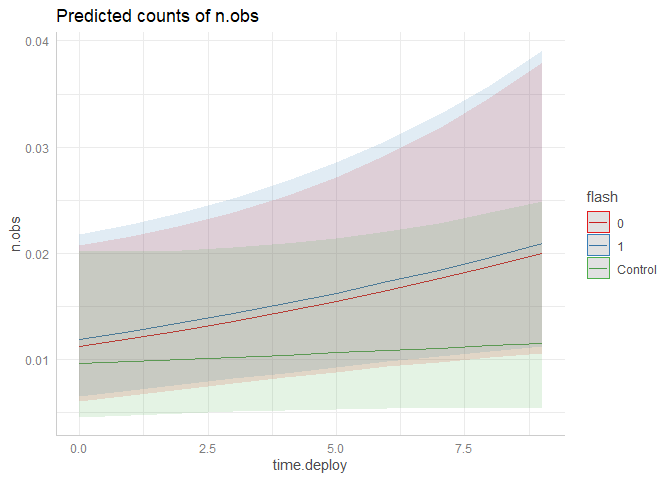
\includegraphics[width=.8\linewidth]{../R/glmm_sp_files/figure-gfm/grevling-report-1.png}
		  \caption{Badger}
		  	\label{fig:glmm_grvl}
	\end{subfigure}
		\begin{subfigure}{.5\textwidth}
		  \centering
		  	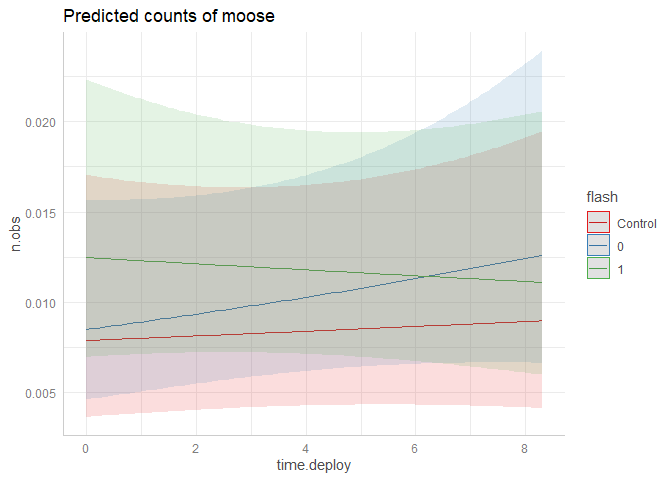
\includegraphics[width=.8\linewidth]{../R/glmm_sp_files/figure-gfm/elg-report-1.png}
		  \caption{Moose}
		  	\label{fig:glmm_elg}
	\end{subfigure}
		\begin{subfigure}{.5\textwidth}
		  \centering
		  	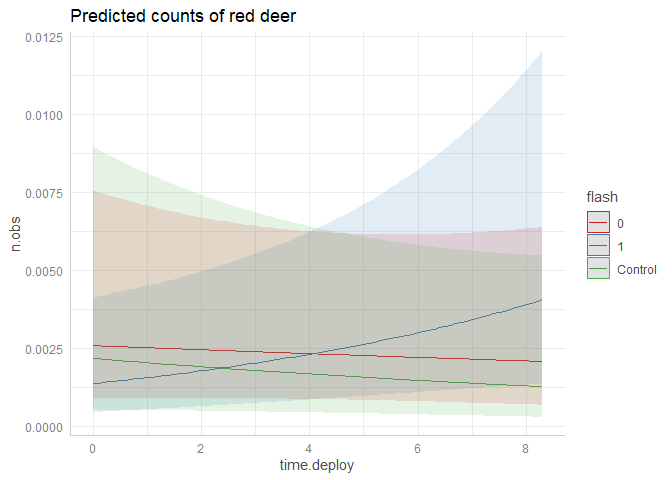
\includegraphics[width=.8\linewidth]{../R/glmm_sp_files/figure-gfm/hjort-report-1.png}
		  \caption{Red deer}
		  	\label{fig:glmm_hjort}
	\end{subfigure}
		\begin{subfigure}{.5\textwidth}
		  \centering
		  	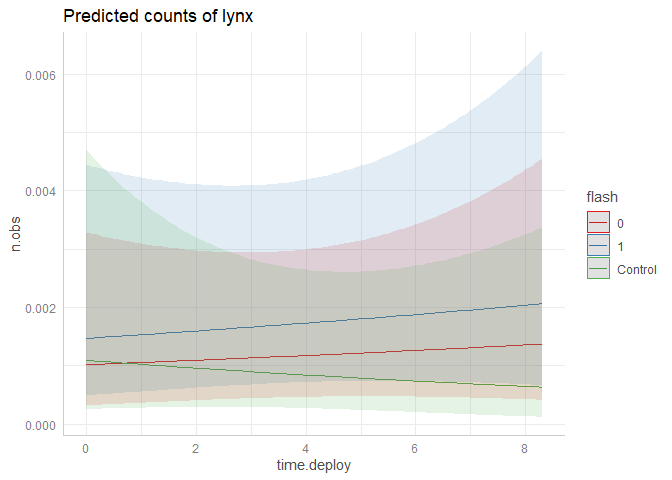
\includegraphics[width=.8\linewidth]{../R/glmm_sp_files/figure-gfm/gaupe-report-1.png}
		  \caption{Lynx}
		  	\label{fig:glmm_gaup}
	\end{subfigure}
		\caption{Fitted GLMM model to each species}
	\label{fig:glmm_sp}
\end{figure}



\begin{figure}
		\begin{subfigure}{.4\textwidth}
		  \centering
	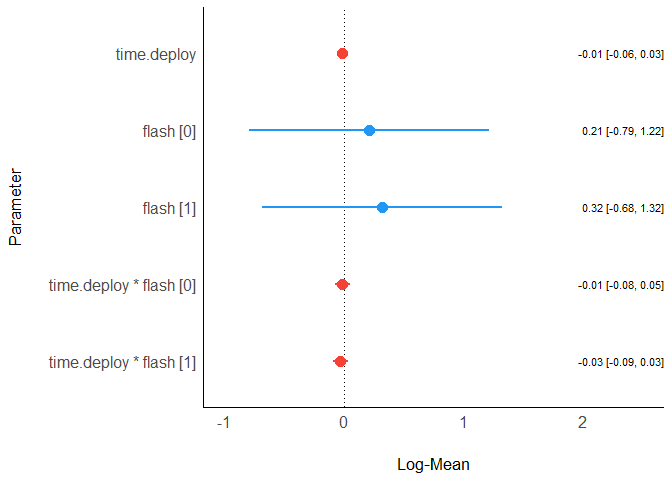
\includegraphics[scale=.4]{../R/glmm_sp_files/figure-gfm/parameters-1.png}
\caption{Intercept included}
		\label{fig:para_raa1}
	\end{subfigure}
		\begin{subfigure}{.4\textwidth}
		  \centering
	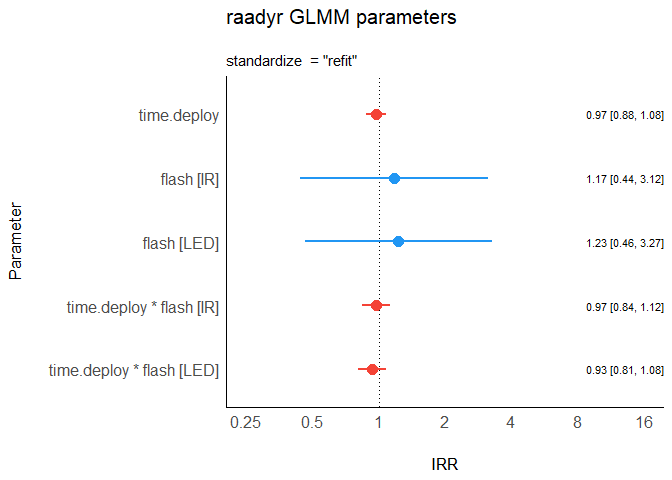
\includegraphics[scale=.4]{../R/glmm_sp_files/figure-gfm/parameters-2.png}
\caption{with values printed}
		\label{fig:para_raa2}
	\end{subfigure}
		\begin{subfigure}{.8\textwidth}
		  \centering
	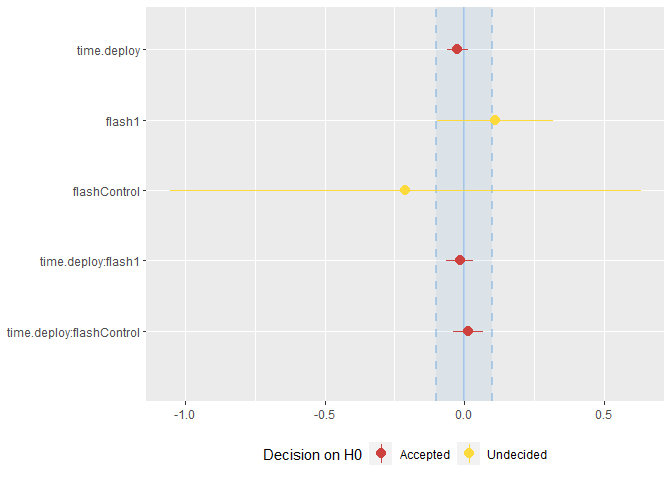
\includegraphics[scale=1]{../R/glmm_sp_files/figure-gfm/parameters-3.png}
\caption{Equivalence test}
		\label{fig:para_raa3}
	\end{subfigure}
		\caption{Visualising model parameters}
	\label{fig:para_sp}
\end{figure}




% On interpretation of relative risks / Incidence rate ratios (which is pretty similar to the coxph)
%https://sphweb.bumc.bu.edu/otlt/mph-modules/ep/ep713_association/ep713_association3.html

\clearpage %to force the insertion of parameters table

\section{Roe deer}

\begin{figure}
\centering
	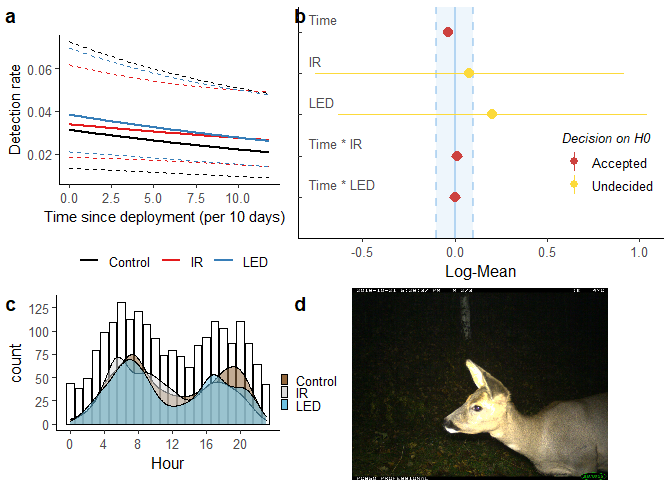
\includegraphics[scale=.9]{../R/glmm_sp_files/figure-html/parameters-1.png}
\caption[Roe deer]
{Roe deer %\par \small
 a) The predicted detection rate of roe deer for each level of the flash-variable. Confidence intervals (CI) represented by dotted lines.\\
b) Model parameters presented in an equivalence test. ROPE is set to $\pm$0.1 Log-Mean, $CI =1 - 2\times \alpha$.\\ 
c) Bars represent the raw count of total roe deer detections per hour of the day, and density curves show the overall pattern for each group.\\
d) LED-CT photograph of a roe deer. The deer passed the camera repeatedly and often stopped in front of the flashing light}\label{fig:raadyr}
\end{figure}


For roe deer, the model explaining variation in detection rate has a substantial explanatory power (conditional R2 = 0.45), but the part related to the fixed effects alone (marginal R2) is just 0.002.
In other words, most of the explained variation in detection rate is due to seasonal changes and variation between the different camera sites captured in the random terms.

The main effect of the white LED periods were non-significantly positive compared to the control-group (Intercept).
The same is true for the IR periods, although to a slightly lower extent.
However, along the time since deployment-axis (time.deploy $\ast$ flash [LED]) there was a negative effect, to the extent that after two months the mean detection rate sank below that of the IR periods (see figure \ref{fig:raadyr}a).
Nevertheless, the confidence intervals (CI) of both white LED and IR periods almost completely overlap, and hence, are not significantly different.


When a parameter is within the ROPE in an equivalence test, it signifies that the difference from the Log-mean, and the variance of the parameter, is low enough that we can accept H0, rather than just fail to reject it.

According to this test, white LED is different enough that we cannot conclude on it’s main effect, but it’s trend over time (Time * LED) is practically equivalent to H0. 
In other words, the equivalence test suggests that there is no significant difference in the long run, but there might be an increase in detections right after the day of deployment.
However, the increase could also result from inhereting a slightly higher detection rate from the IR periods \emph{if} there truly is a negative effect of the white LED over long periods of time.



\newpage
\section{Red fox}

\begin{figure}
		  \centering
	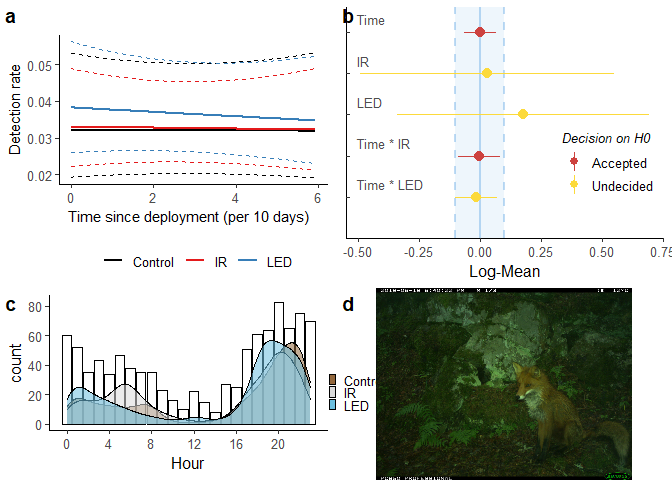
\includegraphics[scale=.9]{../R/glmm_sp_files/figure-html/rev2-1.png}
\caption[Red fox]
{Red fox \par \small 
a) The predicted detection rate of red foxes for each level of the flash-variable. Confidence intervals (CI) represented by dotted lines.\\ 
b) Model parameters presented in an equivalence test. ROPE is set to $\pm$0.1 Log-Mean, $CI =1 - 2\times \alpha$.\\ 
c) Bars represent the raw count of total fox detections per hour of the day, and density curves show the overall pattern for each group.\\
d) LED-CT photograph of a red fox. The fox stopped in front of the flashing camera and waited for a following individual before they continued.}\label{fig:rev}
\end{figure}


For red fox, the model explaining variation in detection rate has a moderate explanatory power (conditional R2 = 0.19), and the part related to the fixed effects alone (marginal R2) is just 0.001. 


The main effect of the white LED periods were non-significantly positive (flash[LED] in table \ref{tab:param}) compared to the IR- and control-periods (flash[IR];Intercept) .
However, along the time since deployment-axis (time.deploy $\ast$ flash [LED]) there was a negative effect, to the extent that after two months the mean detection rate sank below that of the IR periods (see figure \ref{fig:raadyr}a).
Nevertheless, CI of both white LED and IR periods almost completely overlap, and hence, are not significantly different.


\newpage
\section{Badger}


\begin{figure}
		  \centering
	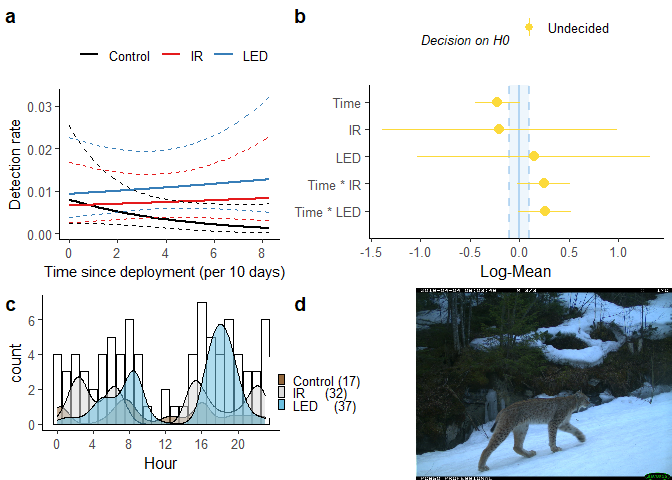
\includegraphics[scale=.9]{../R/glmm_sp_files/figure-html/gaupe2-1.png}
\caption[Lynx]
{Lynx \par \small 
a) The predicted detection rate of lynx for each level of the flash-variable. Confidence intervals (CI) represented by dotted lines.\\ 
b) Model parameters presented in an equivalence test. ROPE is set to $\pm$0.1 Log-Mean, $CI =1 - 2\times \alpha$.\\ 
c) Bars represent the raw count of total lynx detections per hour of the day, and density curves show the overall pattern for each group.\\ 
d) LED-CT photograph of a lynx. DESCRIPT}\label{fig:gaupe}
\end{figure}





\newpage
\section{Hare}

\begin{figure}
		  \centering
	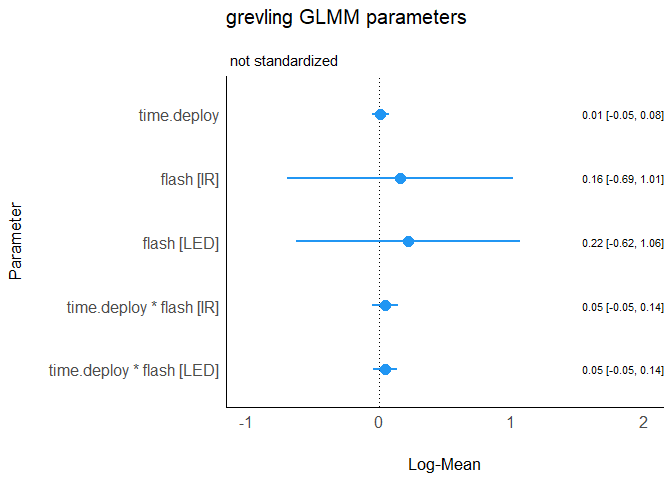
\includegraphics[scale=.9]{../R/glmm_sp_files/figure-html/grevling2-1.png}
\caption[Badger]
{Badger \par \small 
a) The predicted detection rate of badgers for each level of the flash-variable. Confidence intervals (CI) represented by dotted lines.\\ 
b) Model parameters presented in an equivalence test. ROPE is set to $\pm$0.1 Log-Mean, $CI =1 - 2\times \alpha$.\\ 
c) Bars represent the raw count of total badger detections per hour of the day, and density curves show the overall pattern for each group.\\ 
d) LED-CT photograph of a badger. DESCRIPT}\label{fig:grevling}
\end{figure}

For badger, the model explaining variation in detection rate has a substantial explanatory power (conditional R2 = 0.42), but the part related to the fixed effects alone (marginal R2) is just 0.006.




\newpage
\section{Red squirrel}
\section{Moose}

\begin{figure}
		  \centering
	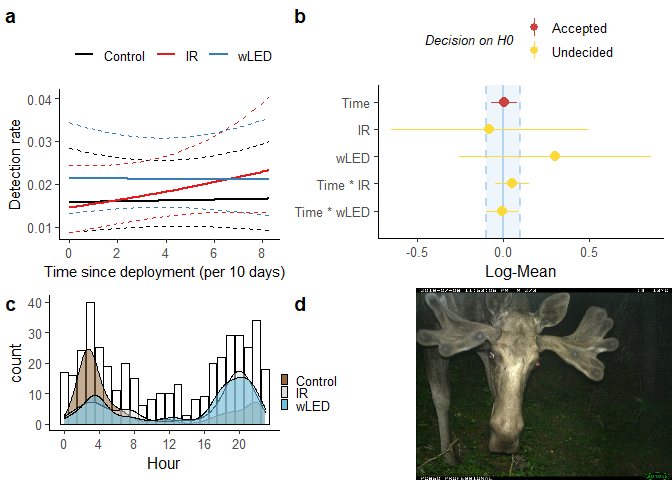
\includegraphics[scale=.9]{../R/glmm_sp_files/figure-html/elg2-1.png}
\caption[Moose]
{Moose \par \small 
a) The predicted detection rate of moose for each level of the flash-variable. Confidence intervals (CI) represented by dotted lines.\\
b) Model parameters presented in an equivalence test. ROPE is set to $\pm$0.1 Log-Mean, $CI =1 - 2\times \alpha$.\\
c) Bars represent the raw count of total detections per hour of the day, and density curves show the overall pattern for each group\\
d) LED-CT photograph of a Moose. DESCRIPT}\label{fig:elg}
\end{figure}


\newpage
\section{Red deer}

\begin{figure}
		  \centering
	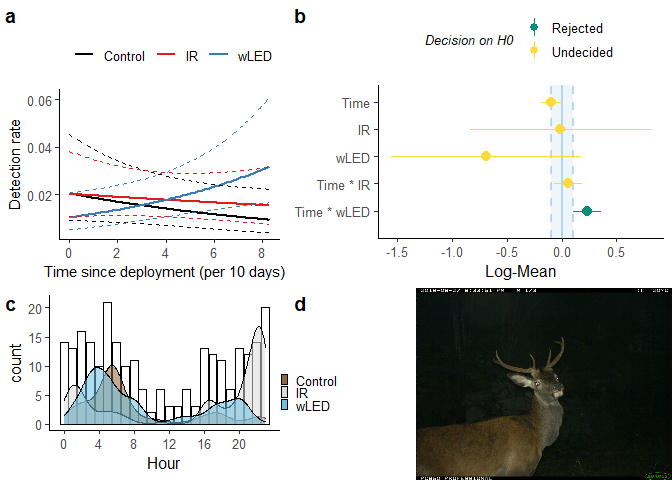
\includegraphics[scale=.9]{../R/glmm_sp_files/figure-html/hjort2-1.png}
\caption[Red deer]
{Red deer \par \small 
a) The predicted detection rate of red deer for each level of the flash-variable. Confidence intervals (CI) represented by dotted lines.\\
b) Model parameters presented in an equivalence test. ROPE is set to $\pm$0.1 Log-Mean, $CI =1 - 2\times \alpha$.\\ 
c) Bars represent the raw count of total Red deer detections per hour of the day, and density curves show the overall pattern for each group.\\ 
d) LED-CT photograph of a red deer. DESCRIPT}\label{fig:hjort}
\end{figure}



\newpage

\begin{figure}
		  \centering
	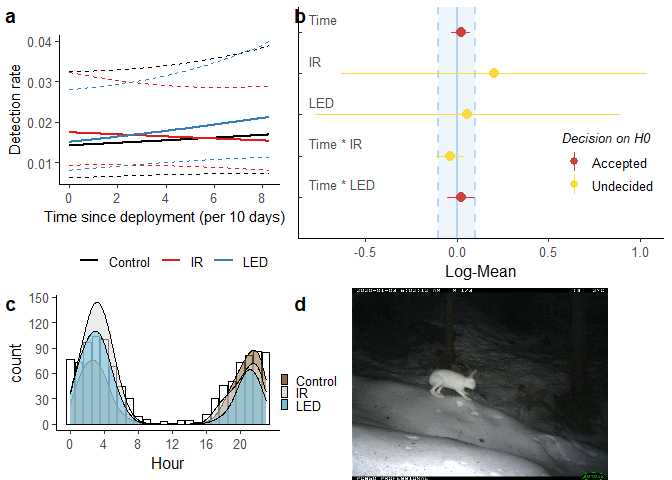
\includegraphics[scale=.9]{../R/glmm_sp_files/figure-html/hare2-1.png}
\caption[Hare]
{Hare \par \small 
a) The predicted detection rate of hares for each level of the flash-variable. Confidence intervals (CI) represented by dotted lines.\\ 
b) Model parameters presented in an equivalence test. ROPE is set to $\pm$0.1 Log-Mean, $CI =1 - 2\times \alpha$.\\ 
c) Bars represent the raw count of total hare detections per hour of the day, and density curves show the overall pattern for each group.\\ 
d) LED-CT photograph of a hare. DESCRIPT}\label{fig:hare}
\end{figure}






\newpage
\section{Pine marten}

\begin{figure}
		  \centering
	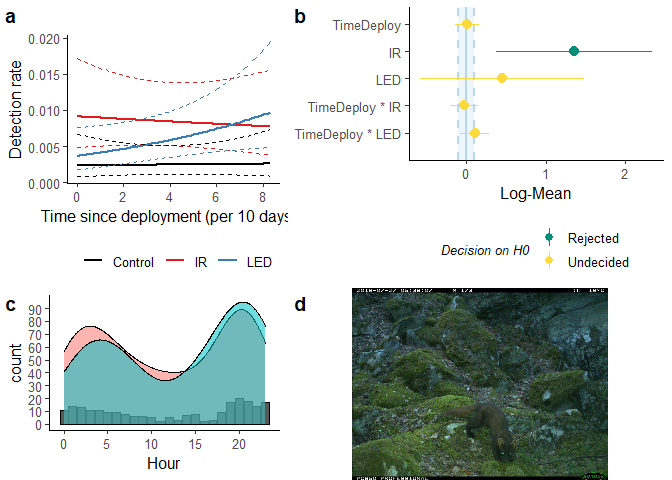
\includegraphics[scale=.9]{../R/glmm_sp_files/figure-html/maar2-1.png}
\caption[Pine marten]
{Pine marten \par \small 
a) The predicted detection rate of pine martens for each level of the flash-variable. Confidence intervals (CI) represented by dotted lines.\\ 
b) Model parameters presented in an equivalence test. ROPE is set to $\pm$0.1 Log-Mean, $CI =1 - 2\times \alpha$.\\ 
c) Bars represent the raw count of total pine marten detections per hour of the day, and density curves show the overall pattern for each group.\\ 
d) LED-CT photograph of a pine marten. DESCRIPT}\label{fig:maar}
\end{figure}






\newpage
\section{Lynx}






% -- discussion --
%\chapter{Discussion}

\section{GLMM}

The intercept-value is considered significantly negative, which is to say that there were a low chance of detecting any roe deer at an IR-camera the same day I visited the camera (see figure \ref{fig:para_raa1}). 

This makes intuitive sence, as most large mammals would be scared away temporarily by a nearby human, especially the times i set up the additional camera boxes, which I did with an electrical drill.

Anecdotally, once I saw a roe deer about to walk by a CT when I came to inspect it. The roe deer saw me and fled, right before it was detected by the camera. I've also startled two badgers close by a CT. However, they didn't run far away, and went on to repopulate the area quickly.
Chances are I’ve scared animals other times as well, but haven’t noticed it.

The effect of time since deployment is non-significant, and $\beta = 0.007$.
That means there is no difference on the baseline detection rate for an IR camera over time (after controlling for seasonal changes).

For white LED flash $\beta = 0.04$, meaning that the intercept is slightly higher than for IR, but the difference is non-significant.

The control-group has practically the same intercept as the IR-groups, and all of the groups is showing a negative trend, non-significant trend over time. The negative trends for the control- and IR-groups are strange, as they should represent a baseline detection probability, and any fluctuations in detection rates over the year should be controlled for by the weekly random effect-argument.

Seeing as all the parameters related to time since deployment are well within the ROPE area in figure \vref{fig:para_raa3} (/ all have a non-significant p-value), it is safe to say that these "trends" are only due to chance. 

The raw count-plots in Appendix A also shows that there are more outliers with extreme values (counts of up to 5 events per day) when time since deployment is close to 0, than towards the maximum lengths of periods. The largest counts stem from the control-group which in mainly has arbitrary days set as their day 0 in each period. Only a few cameras has a true visitation date as their day 0, which can be seen as their first point after a gap in figure \ref{fig:timeseries_control}.


Hypothesising:

\textbf{If} $H_1$ is true, and there truly is an effect of the white LED for long periods on the detection rate of roe deer, this effect could in turn account for the different intercept values of IR and flash, as the IR periods usually starts after a flash period (with the exception of the first IR-period, i.e. first red periods in figure \vref{fig:timeseries_flash}).

Remembering my study design, 20 cameras start with white LED, 20 with IR.
Intercept should theoretically be identical in the 1st period.
2nd period; white LEDs are moved. New LED CTs should have same intercept (unchanged detection rate), and new IR CTs should have a hypothetical lower intercept due to the effect of white LED.
3rd period; white LED moved, new LED CTs (IR intercept), new IR CTs (hypothetical lower intercept), and so on.

Which sums up to 3 IR periods where detection rates could start lower than that of white LED.

If that was true, and the white LED interacting with time had a significantly negative slope, then the slope of IR should be positive, as the roe deer detection rate returned to normal.
The slope for the control-group(time.deploy:flashControl) should represent a normal detection rate, and be close to flat ($ \beta \approx 0$), intercept possibly closer to that of white LED, than IR.


\section*{Kommentar}

Om "Hypothesising"-delen skal med på noko vis må den heilt klart skrivast om, men eg inkluderte den foreløpig for å høyre om du synst den har ein plass i diskusjons-delen ein eller annan plass.

I tillegg er mesteparten av skrift her truleg overflødig, men eg skreiv den simultant med modelleringa for at eg skulle forstå meg sjølv igjen etter at det hadde gått nokon dager. Kor utdypande er det verdt å gå i detaljnivået her?  Burde eg droppe å utdype ting som likevel ikkje er signifikant?


%POST-IT
%% Physiological features of species could determine effect: badgers poor eye sight -> less reactive to visual stimuli?
%%Species interaction with human: high conflict animals wary of flash as it signals humans nearby
%%Camera site proximity to urban area/ roads (Artificial Light At Night) : +correlation with proximity and effect on species
%%smaller animals less likely to be detected by camera. Dark numbers?









% -- conclusion --
%\chapter{Conclusion}



% -- appendix --
%\appendix
%\section*{Appendices}
%\addcontentsline{toc}{section}{Appendices}
%\renewcommand{\thesubsection}{\Alph{subsection}}
%
%\subsection{R Session Info}
%\label{app:sessinfo}

%\begin{table}

\caption[ ]{(ref:Reproducibility-SessionInfo-R-packages-title)}
\centering
\begin{tabular}[t]{lll}
\toprule
Package & Loaded version & Date\\
\midrule
broom & 0.7.3 & 2020-12-16\\
devtools & 2.3.2 & 2020-09-18\\
dials & 0.0.9 & 2020-09-16\\
dplyr & 1.0.3 & 2021-01-15\\
equatiomatic & 0.1.0 & 2020-08-27\\
\addlinespace
forcats & 0.5.0 & 2020-03-01\\
ggplot2 & 3.3.3 & 2020-12-30\\
ggpubr & 0.4.0 & 2020-06-27\\
infer & 0.5.4 & 2021-01-13\\
kableExtra & 1.3.1 & 2020-10-22\\
\addlinespace
lubridate & 1.7.9.2 & 2020-11-13\\
magrittr & 2.0.1 & 2020-11-17\\
modeldata & 0.1.0 & 2020-10-22\\
pander & 0.6.3 & 2018-11-06\\
parsnip & 0.1.5 & 2021-01-19\\
\addlinespace
purrr & 0.3.4 & 2020-04-17\\
readr & 1.4.0 & 2020-10-05\\
recipes & 0.1.15 & 2020-11-11\\
report & 0.2.0 & 2021-01-28\\
rsample & 0.0.8 & 2020-09-23\\
\addlinespace
scales & 1.1.1 & 2020-05-11\\
stringr & 1.4.0 & 2019-02-10\\
survival & 3.2-7 & 2020-09-28\\
survminer & 0.4.8 & 2020-07-25\\
tibble & 3.0.5 & 2021-01-15\\
\addlinespace
tidymodels & 0.1.2 & 2020-11-22\\
tidyr & 1.1.2 & 2020-08-27\\
tidyverse & 1.3.0 & 2019-11-21\\
tune & 0.1.2 & 2020-11-17\\
usethis & 2.0.0 & 2020-12-10\\
\addlinespace
vip & 0.3.2 & 2020-12-17\\
workflows & 0.2.1 & 2020-10-08\\
yardstick & 0.0.7 & 2020-07-13\\
\bottomrule
\end{tabular}
\end{table}


%\subsection{\\Another Appendix}



%This is a reference to the session info appendix \ref{app:sessinfo}
\appendix
%\begin{appendices} %Seems I don't need this because of the \appendix command 

\section{\\Title of Appendix A}
\label{app:sessinfo}
This is the session info appendix...
\begin{table}

\caption[ ]{(ref:Reproducibility-SessionInfo-R-packages-title)}
\centering
\begin{tabular}[t]{lll}
\toprule
Package & Loaded version & Date\\
\midrule
broom & 0.7.3 & 2020-12-16\\
devtools & 2.3.2 & 2020-09-18\\
dials & 0.0.9 & 2020-09-16\\
dplyr & 1.0.3 & 2021-01-15\\
equatiomatic & 0.1.0 & 2020-08-27\\
\addlinespace
forcats & 0.5.0 & 2020-03-01\\
ggplot2 & 3.3.3 & 2020-12-30\\
ggpubr & 0.4.0 & 2020-06-27\\
infer & 0.5.4 & 2021-01-13\\
kableExtra & 1.3.1 & 2020-10-22\\
\addlinespace
lubridate & 1.7.9.2 & 2020-11-13\\
magrittr & 2.0.1 & 2020-11-17\\
modeldata & 0.1.0 & 2020-10-22\\
pander & 0.6.3 & 2018-11-06\\
parsnip & 0.1.5 & 2021-01-19\\
\addlinespace
purrr & 0.3.4 & 2020-04-17\\
readr & 1.4.0 & 2020-10-05\\
recipes & 0.1.15 & 2020-11-11\\
report & 0.2.0 & 2021-01-28\\
rsample & 0.0.8 & 2020-09-23\\
\addlinespace
scales & 1.1.1 & 2020-05-11\\
stringr & 1.4.0 & 2019-02-10\\
survival & 3.2-7 & 2020-09-28\\
survminer & 0.4.8 & 2020-07-25\\
tibble & 3.0.5 & 2021-01-15\\
\addlinespace
tidymodels & 0.1.2 & 2020-11-22\\
tidyr & 1.1.2 & 2020-08-27\\
tidyverse & 1.3.0 & 2019-11-21\\
tune & 0.1.2 & 2020-11-17\\
usethis & 2.0.0 & 2020-12-10\\
\addlinespace
vip & 0.3.2 & 2020-12-17\\
workflows & 0.2.1 & 2020-10-08\\
yardstick & 0.0.7 & 2020-07-13\\
\bottomrule
\end{tabular}
\end{table}



\section{\\Another Appendix}

%\end{appendices}

 %maybe forget about this one

\clearpage
\printbibliography

\end{document}

